\chapter{分形BBH模型理论}
高阶拓扑绝缘体(HOTIs)是一种新近发展的拓扑相,它承载着低维度的更高余维拓扑态,这些态局域在“边界的边界”上\cite{benalcazar2017quantized,langbehn2017reflection,song2017d,schindler2018higher,ezawa2018higher,trifunovic2019higher,xie2021higher}。这类新型拓扑相的诱导机制主要包含两种典型途径:其一是基于Benalcazar-Bernevig-Hughes(BBH)四极子绝缘体模型\cite{benalcazar2017quantized},该模型具有量子化的体四极矩但体偶极极化为零。由于扩展的高阶体-边界对应原理,二维体系可同时支持0D带隙角态和1D带隙边缘态。另一种经典方法是将1D SSH模型直接推广到更高维度\cite{noh2018topological,ni2019observation,zhang2019second,xue2019acoustic,zhang2020low}。通过改变2D系统中内部和外部跳跃的相对强度,可以诱导出二阶拓扑相,其拓扑不变量是偶极极化,而不是四极矩。得益于人工晶体设计的灵活性,这些方法在过去十年中极大地推动了HOTIs及传统拓扑绝缘体\cite{hasan2010colloquium,qi2011topological}的研究进程。迄今为止,HOTIs在经典波系统中得到了广泛验证,包括光子学\cite{peterson2018quantized,xie2018second,chen2019direct,xie2019visualization,mittal2019photonic,ota2019photonic,el2019corner,he2020quadrupole,zhang2020higher,li2020higher}、声学\cite{serra2018observation,zhang2019dimensional,xue2019realization,qi2020acoustic,xue2020observation,weiner2020demonstration,ni2020demonstration}和电路系统\cite{imhof2018topolectrical,bao2019topoelectrical,zhang2019dimensional,liu2020octupole,zhang2021experimental}等实验平台,并引领了与非厄米性\cite{luo2019higher,gao2021non}、无序\cite{zhang2021experimental,chen2020higher,li2020topological}和非线性\cite{zangeneh2019nonlinear,kirsch2021nonlinear}相互作用等新兴研究领域。

另一方面,分形体系中的拓扑态研究也取得了显著进展\cite{song2014topological,iliasov2020hall,fremling2020existence,yang2020photonic},分形结构以其独特的自相似性和分数维度特征\cite{mandelbrot1967coast},为探索新型拓扑物态提供了新的平台。近期研究表明,具有外角和内角模式的量子分形中可能存在高阶拓扑相\cite{pai2019topological,manna2022higher},这为分形与HOTIs的交叉研究架起了桥梁。然而,高阶拓扑相与分形晶格的相互作用机制仍处于初期探索阶段。

在本章,笔者实现了一个分形晶格的高阶拓扑相。本文将 BBH 模型应用于1.89 维 Sierpinski 地毯。基于实空间多体多极算符\cite{wheeler2019many,kang2019many}计算了相图的相图计算表明,分形特性使四极子相的非平庸区域压缩了0.35倍。在拓扑相区域内,精确对角化哈密顿量得到的能谱呈现出分形“蝴蝶”结构,包含丰富的外角态和不同的内角态。通过分数量子化电荷计算\cite{li2020fractional,peterson2021trapped,liu2021bulk},我们证实了外角态和内角态均具有拓扑非平庸特性。通过遍历所有晶格点,我们发现了外角和内角处丰富的拓扑角态,其维度分别对应于 0 和 1.89。角态的分数维度此前从未被报道,因此使得我们的分形拓扑绝缘体与传统拓扑绝缘体明显不同。
\section{分形BBH模型的紧束缚模型}
\subsection{分形晶格与BBH模型的哈密顿量}
本文采用的承载高阶拓扑绝缘体的分形晶格为Sierpinski地毯,如图\ref{fig:Generation}所示。晶格由一个四格点的正方形为基本单元,通过迭代生成。
\begin{figure}[htbp]
    \centering
    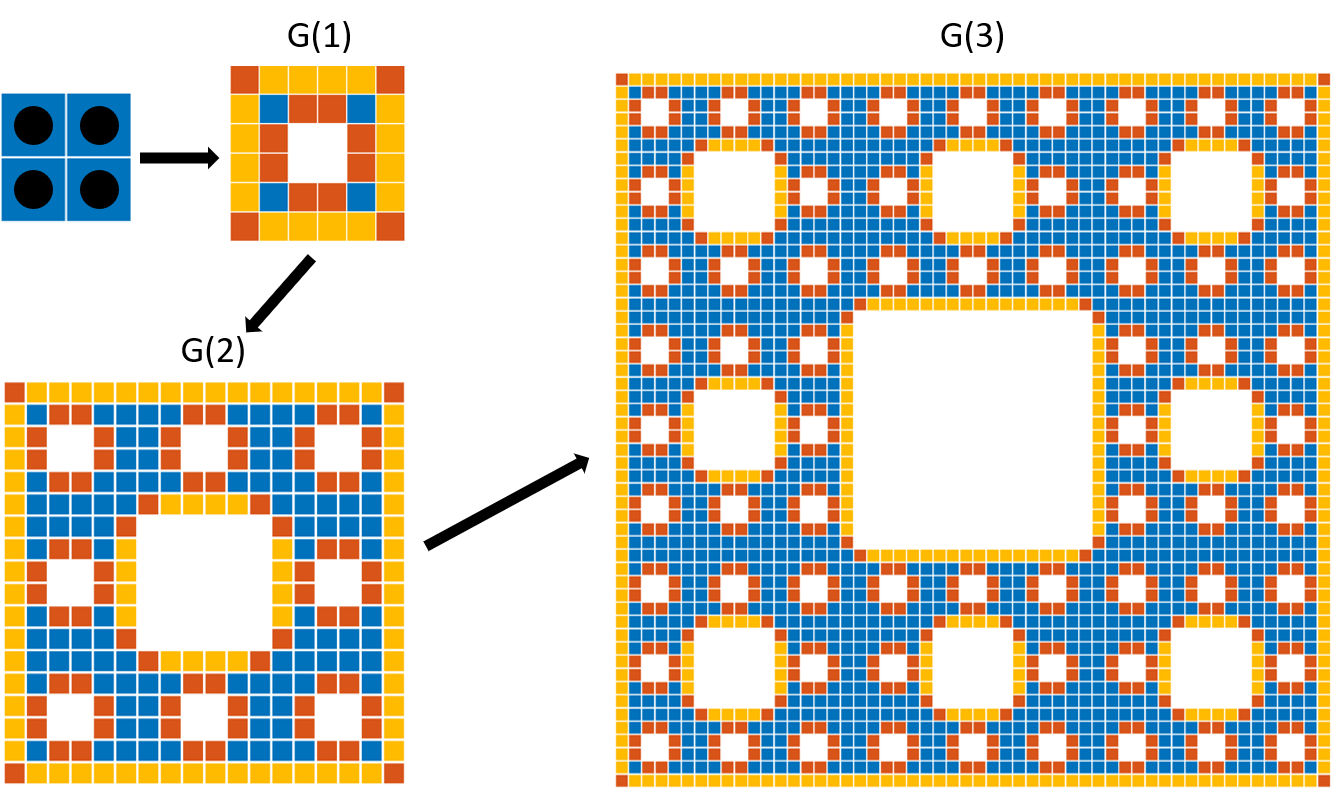
\includegraphics[width=0.75\linewidth]{figure/HOTITheo/Generation.png}
    \caption{分形晶格的迭代生成}分形晶格及拓扑态的维度。晶格的最小元胞包含四个原子(黑点)。Sierpinski 地毯的第 \( n \) 代 G(n) 由 G(n-1) 的八个副本组成。紫色、红色、黄色和蓝色框分别表示外角、内角、边缘和“体”格点。
    \label{fig:Generation}
\end{figure}

我们基于Sierpinski地毯的分形模型如图\ref{fig:HOTIlattice}(a)所示。最小原胞由BBH模型的晶胞构成,如图\ref{fig:HOTIlattice}(b)所示。细线和粗线分别表示内部跳跃$t_1$和外部跳跃$t_2$,红色(绿色)线表示正(负)耦合,从而可以为每个格子引入有效的磁通量$\phi=\pi$。

\begin{figure}[htbp]
    \centering
    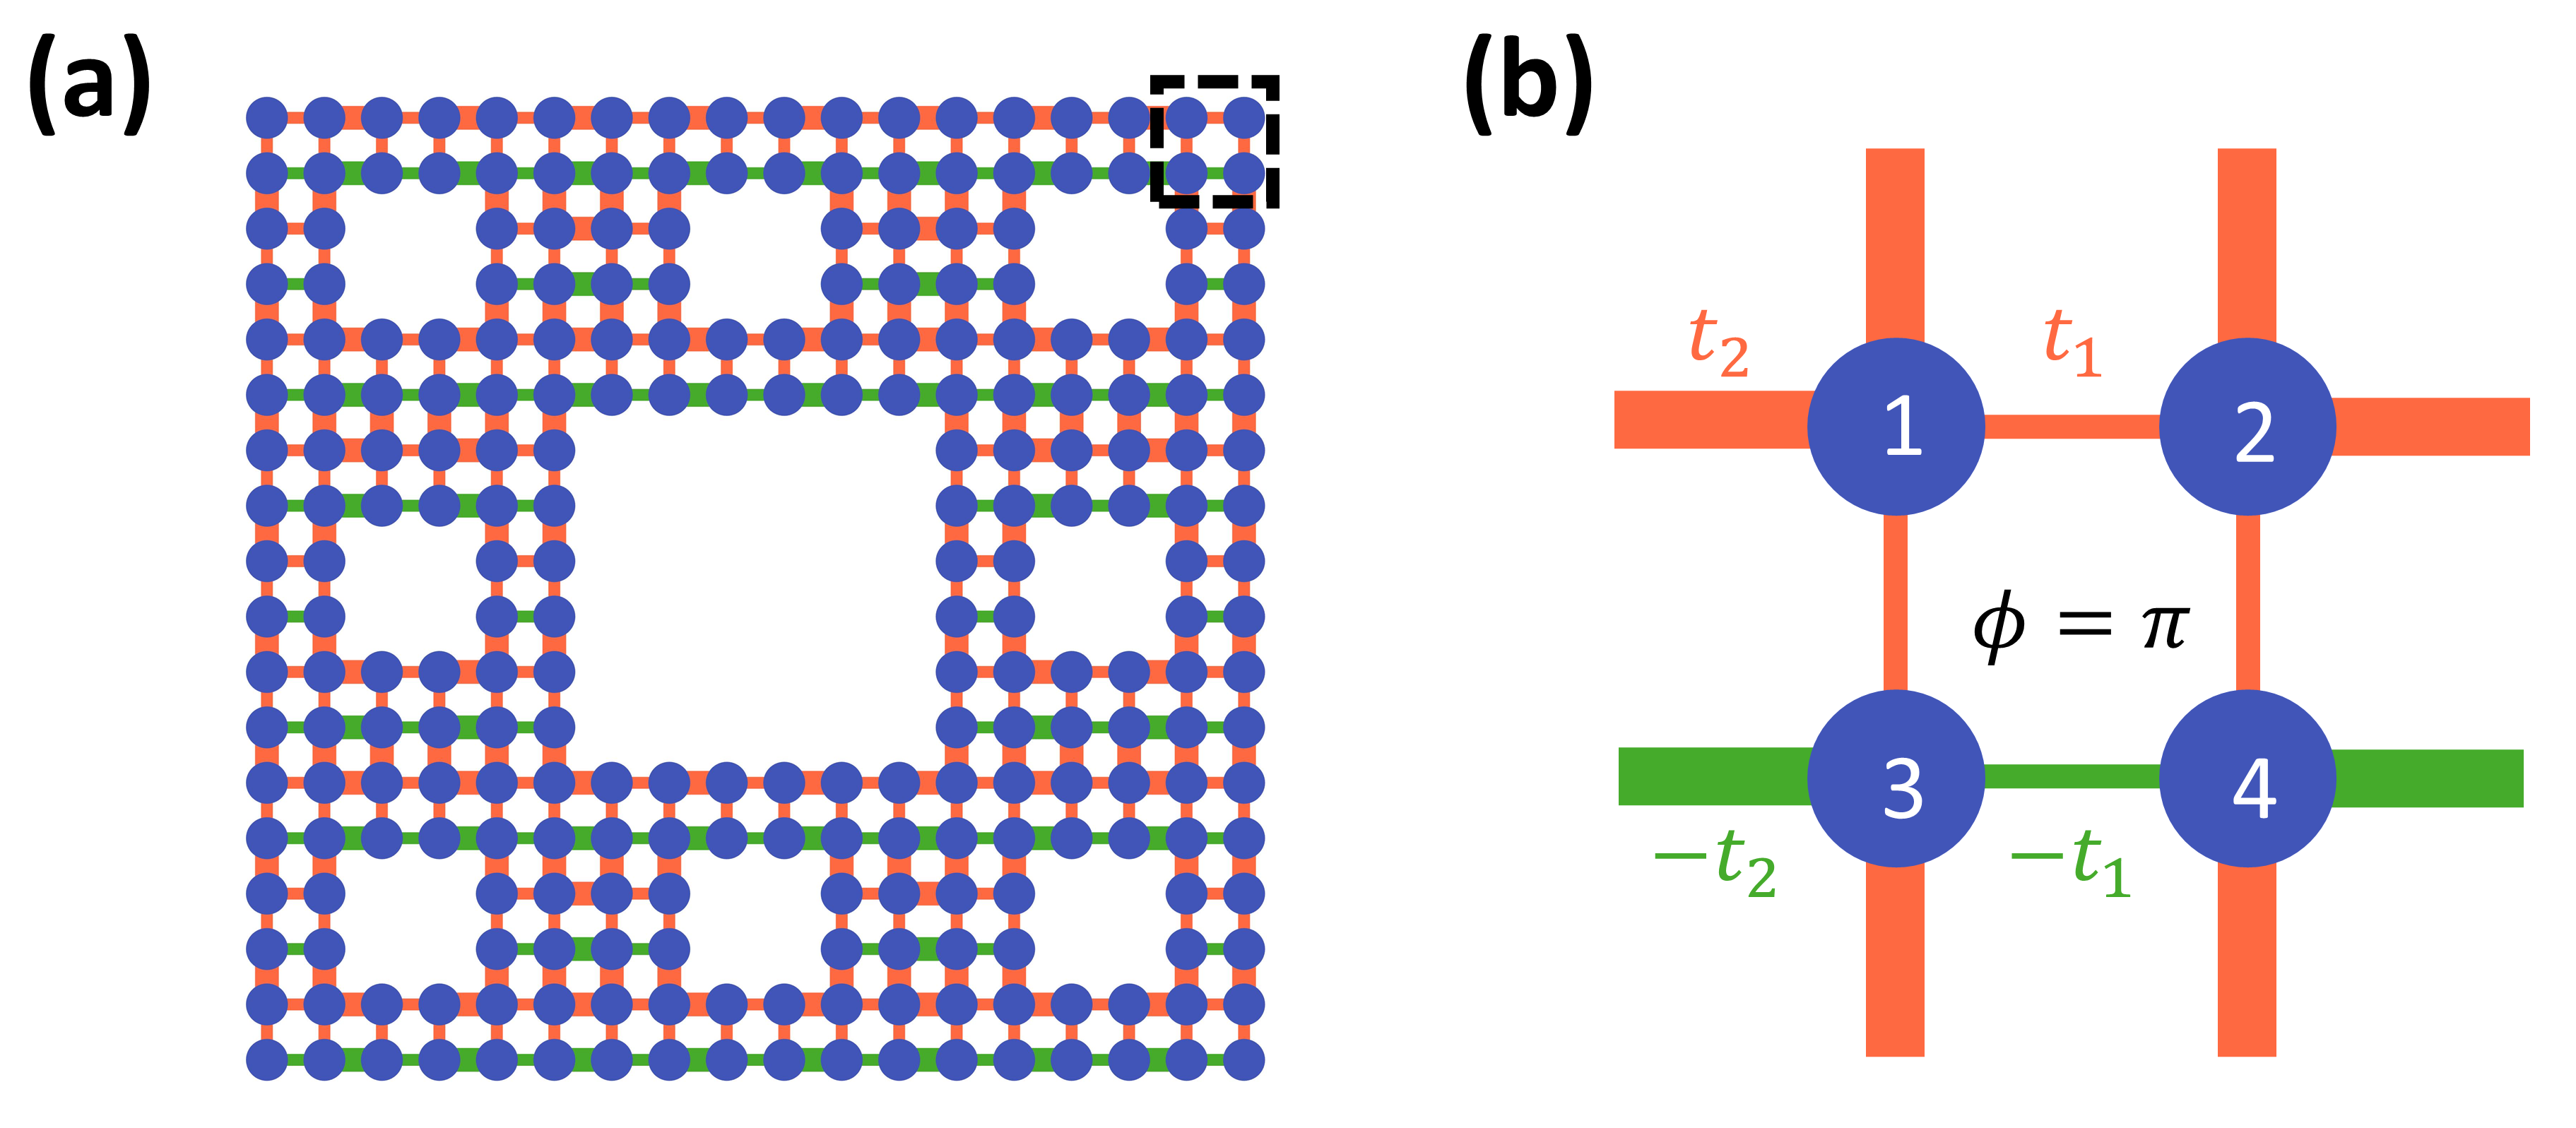
\includegraphics[width=0.5\linewidth]{figure/HOTITheo/HOTIlattice.png}
    \caption{分形晶格与耦合}(a) 分形Sierpinski地毯的示意图。细线(粗线)表示强度为内部(外部)跳跃$t_1$($t_2$)的跳跃,而红色(绿色)线表示正(负)跳跃。虚线框的放大视图如图(b)所示。
    \label{fig:HOTIlattice}
\end{figure}

在该系统中,紧束缚模型下的哈密顿量可以表示为:
\begin{equation}
\hat{H} = \sum_\text{intra} c_i^\dagger H_\text{intra} c_i + \sum_\text{inter} c_j^\dagger H_\text{inter} c_j,
\end{equation}
其中
\begin{equation}
\begin{aligned}
H_\text{intra} = & \, t_1 (\sigma_x \otimes I + I \otimes \tau_x + \sigma_y \otimes \tau_y), \\
H_\text{inter} = & \, t_2 (\sigma_x \otimes I + I \otimes \tau_x + \sigma_y \otimes \tau_y).
\end{aligned}
\end{equation}
其中,\( \hat{c}_i^\dagger \)(\( \hat{c}_i \))为位于第 \( i \) 站点的产生(湮灭)算符,如图 1(a) 所示。矩阵 \( H_{\text{intra}} \)(\( H_{\text{inter}} \))分别描述了 BBH 模型中的站点内跳跃和站点间跳跃。

为了产生量子化的四极矩,需要对站点内跳跃和站点间跳跃进行偶极化耦合,这些跳跃由 \( t_1 \) 和 \( t_2 \) 表示。在我们的分形模型中,该系统保持了时间反演对称性、粒子-空穴对称性和手性对称性,但破坏了平移对称性。

\subsection{BBH模型的拓扑不变量}
在一阶拓扑绝缘体中,拓扑不变量起源于Berry相位的奇点。而高阶拓扑绝缘体的拓扑来源于拓展的高阶Berry相。高阶 Berry 相位是拓扑物理中研究高阶拓扑绝缘体的重要工具之一。它扩展了标准 Berry 相位的概念,用于刻画高阶拓扑不变量,例如四极子(quadrupole)、八极子(octupole)拓扑相等。

Berry 相位是量子系统在参数空间(如动量空间)中绝热变化所累积的几何相位: 
\begin{equation}
    \gamma = \oint_{\mathcal{C}} \mathbf{A} \cdot d\mathbf{k},
\end{equation}
其中,\( \mathbf{A}(\mathbf{k}) \) 为 Berry 连接$\mathbf{A}(\mathbf{k}) = i \langle u(\mathbf{k}) | \nabla_{\mathbf{k}} | u(\mathbf{k}) \rangle$。
对于二维系统,拓扑不变量Chern 数可以用 Berry 曲率积分计算: 
\begin{equation}
    C = \frac{1}{2\pi} \int_{\text{BZ}} d^2k \, \Omega(\mathbf{k}),
\end{equation}
其中,Berry 曲率定义为$\Omega(\mathbf{k}) = \nabla_{\mathbf{k}} \times \mathbf{A}(\mathbf{k})$。

在传统拓扑绝缘体中,Berry 相位用于计算 Chern 数、Zak 相位等拓扑不变量。 对于高阶拓扑绝缘体,拓扑性质通常不能由 Chern 数刻画,而需要引入高阶 Berry 相位。特别地,在本文的BBH模型中,四极子拓扑不变量可以通过高阶 Berry 相位计算。

计算高阶 Berry 相位通常使用嵌套 Wilson 环方法:在某个方向上先计算 Wilson 环矩阵$W_x(k_y)$ 并得到其本征值 $\theta_n(k_y)$。接着利用 Wilson 环本征态计算第二个 Wilson 环$W_y^{(\nu)}$ 。最后从 Wilson 环的本征值中提取高阶 Berry 相位。 首先,我们计算沿某一方向(如 \( k_x \))的 Wilson 环:
\begin{equation}
    W_x(k_y) = P e^{i \oint A_x \cdot dk_x}。
\end{equation}
该 Wilson 环的本征值提供了极化信息 $e^{i\theta_n(k_y)}$。利用从 Wilson 环获得的本征态 \( |\nu_n(k_y)\rangle \),我们计算沿 \( k_y \) 的二阶 Wilson 环:
\begin{equation}
    W_y^{(\nu)} = P e^{i \oint A_y^{(\nu)} \cdot dk_y},
\end{equation}
其中,在此基底中的 Berry 连接为$A_y^{(\nu)} = i \langle \nu_n(k_y) | \nabla_{k_y} | \nu_m(k_y) \rangle$。而高阶 Berry 相位由下式给出:
\begin{equation}
    \gamma^{(2)} = \oint_{\mathcal{C}'} \mathbf{A}^{(1)} \cdot d\mathbf{k}。
\end{equation}
在四极子拓扑绝缘体中,四极子矩与二阶 Berry 相位相关:
\begin{equation}
    q_{xy} = \frac{ \gamma^{(2)}}{2\pi}  \mod 1。
\end{equation}
当 \( q_{xy} = 0.5 \) 时,系统处于四极子拓扑相,并在角落处存在受保护的零能态。

嵌套 Wilson 环与高阶Berry相很好的描述了二维高阶拓扑绝缘体的拓扑。但由于分形晶格缺乏平移对称性,且 Bloch 定理失效,无法直接在k空间计算高阶Berry相。因此需要使用实空间的拓扑不变量。基于多体电多极矩算符的实空间四极矩\cite{wheeler2019many,kang2019many}是一种等价的高阶拓扑不变量。实空间四极矩可以表示为:
\begin{equation}
Q_{xy} = \frac{1}{2\pi} \text{Im} \log \left[ \det \left( U^\dagger \hat{Q} U \right)\sqrt{\det \left(\hat{Q}^\dagger \right)} \right] \mod 1
\end{equation}

其中,\( \hat{Q} = \exp \left[i 2\pi \hat{x} \hat{y}/(L_x L_y) \right] \) 是对角酉矩阵,\( \hat{x} \)(\( \hat{y} \))分别是沿水平方向(垂直方向)的位置算符,\( L_x \)(\( L_y \))是晶格在 \( x \)(\( y \))方向上的长度,\( U \) 是一个矩阵,其列向量是哈密顿量在半填充条件下的本征态。四极矩被量子化为 0 或 1/2,对应于平庸相或高阶拓扑相。在本章的后续内容中,分形晶格的高阶拓扑不变量均通过实空间方案计算。


\section{分形能谱和拓扑态}
在能带拓扑体系中,系统哈密顿量的能谱反应了系统的拓扑性质。系统能隙的打开再开启表明了拓扑相变的位置,此外实空间特征值中,能带中心还会出现相应的拓扑局域态。在本节,笔者计算了谢宾斯基地毯晶格BBH模型的能谱随内部跳跃$t_1$的变化,并将结果展示在图\ref{fig:HOTISpec}(a, b)中。灰色和蓝色曲线分别表示“体态”(晶格内部)和边缘态,这与整数维系统中HOTI的情况相似。在\ref{fig:HOTISpec}(b)中,大量角态在能量谱中心($t_1=0$和$E=0$)相交,并形成分形“蝴蝶”状,这与基于BBH模型的传统HOTI有根本区别。红线表示外部角态,它们在$t_1=-0.35$到$t_1=0.35$范围内简并,其表明了系统的拓扑相区域,如图\ref{fig:HOTISpec}(c)所示。黄色和绿色曲线分别表示两种不同类型的内角态A和B。为简化起见,本章中外部跳跃强度$t_2$设为1。在图\ref{fig:HOTISpec}中,我们用蓝色阴影标记了拓扑相区域。

拓扑相变的一个重要特征是能带的闭合和重新打开。在高阶拓扑绝缘体中,其体现为边缘哈密顿量的能隙关闭再打开。然而,再图\ref{fig:HOTISpec}(a)中,尽管其在$t_1=-0.35$和$t_1=0.35$两点距离最近,对应着拓扑相变的位置,但蓝色的边缘态能隙并未彻底关闭。一方面,由于维度的降低,体态数量的减少导致拓扑相变期间能隙的打开。另一方面,内角态B[图\ref{fig:HOTISpec}(g)]不被晶格的边缘隔开,因此其可能无需边缘态带隙的闭合再打开。从灰色(体态)和蓝色(边缘态)曲线可以看出,在相变期间,能量间隙在-0.9到0.9范围内仍然存在,这使得我们的分形模型与二维BBH模型显著不同。

\begin{figure}[htbp]
    \centering
    \includegraphics[width=1\linewidth]{figure/HOTITheo/HOTISpec.png}
    \caption{分形能谱与拓扑态}(a) 能量谱随内部跳跃$t_1$的变化,其中$t_2=1$。灰色和蓝色曲线分别表示体态和边缘态,而红色、黄色和绿色曲线分别表示外部角态、内部角态A和B。(b) 图(a)中虚线框内分形“蝴蝶”的放大视图。分形晶格中的拓扑态。(c) 固定$t_1/t_2=0.13$时的能量谱,对应于(a)中蓝色虚线。(d)角态的放大视图,对应于(c)中虚线框。(e-h) 外部角态、内部角态A、B以及边缘态的总空间分布。
    \label{fig:HOTISpec}
\end{figure}

在展示了分形“蝴蝶”后,我们进一步探讨分形模型所承载的丰富态。我们在图\ref{fig:HOTISpec}(c)中绘制了固定$t_1/t_2=0.13$时的能量谱,并在图\ref{fig:HOTISpec}(d)中展示了所有角态的放大视图。首先,我们关注四个外部角态(红点),它们在能量为零处简并。这四个态的总分布局域在分形晶格的四个外角,如图\ref{fig:HOTISpec}(e)所示,这是高阶拓扑相的关键特征。其次,如图\ref{fig:HOTISpec}(f, g)所示,存在大量标记为A和B的内部角态,对应于图\ref{fig:HOTISpec}(c)中的黄色和青色点,局域在不同尺寸的内部空洞的角落。需要注意的是,与外部角落跨越$\pi/2$角度不同,分形晶格中的内部角落跨越$3\pi/2$,这导致内部角态均等地分裂到内部空洞角落附近的两个边缘位置。最后,在图\ref{fig:HOTISpec}(h)中,我们展示了与图\ref{fig:HOTISpec}(c)中蓝点对应的边缘态的总分布,分形晶格的边缘态亦同时分布在内外边界。

\subsection{分形晶格的基本单元及其混合}
不难发现,在图\ref{fig:HOTISpec}(a)中,当我们设定$t_1=0$时,角态,边缘态和体态分别简并于能量$E=0$,$E=t_2$和$E=\sqrt{2}t_2$处。将内部耦合调节到$t_1=0$这一过程是绝热的,不会伴随能带关闭或任何拓扑相变。但由于此时不存在内部耦合,分形晶格被分裂为各种基本单元,例如图\ref{fig:Elemen}中所示的单体、二聚体、三聚体和四聚体。

\begin{figure}[htbp]
    \centering
    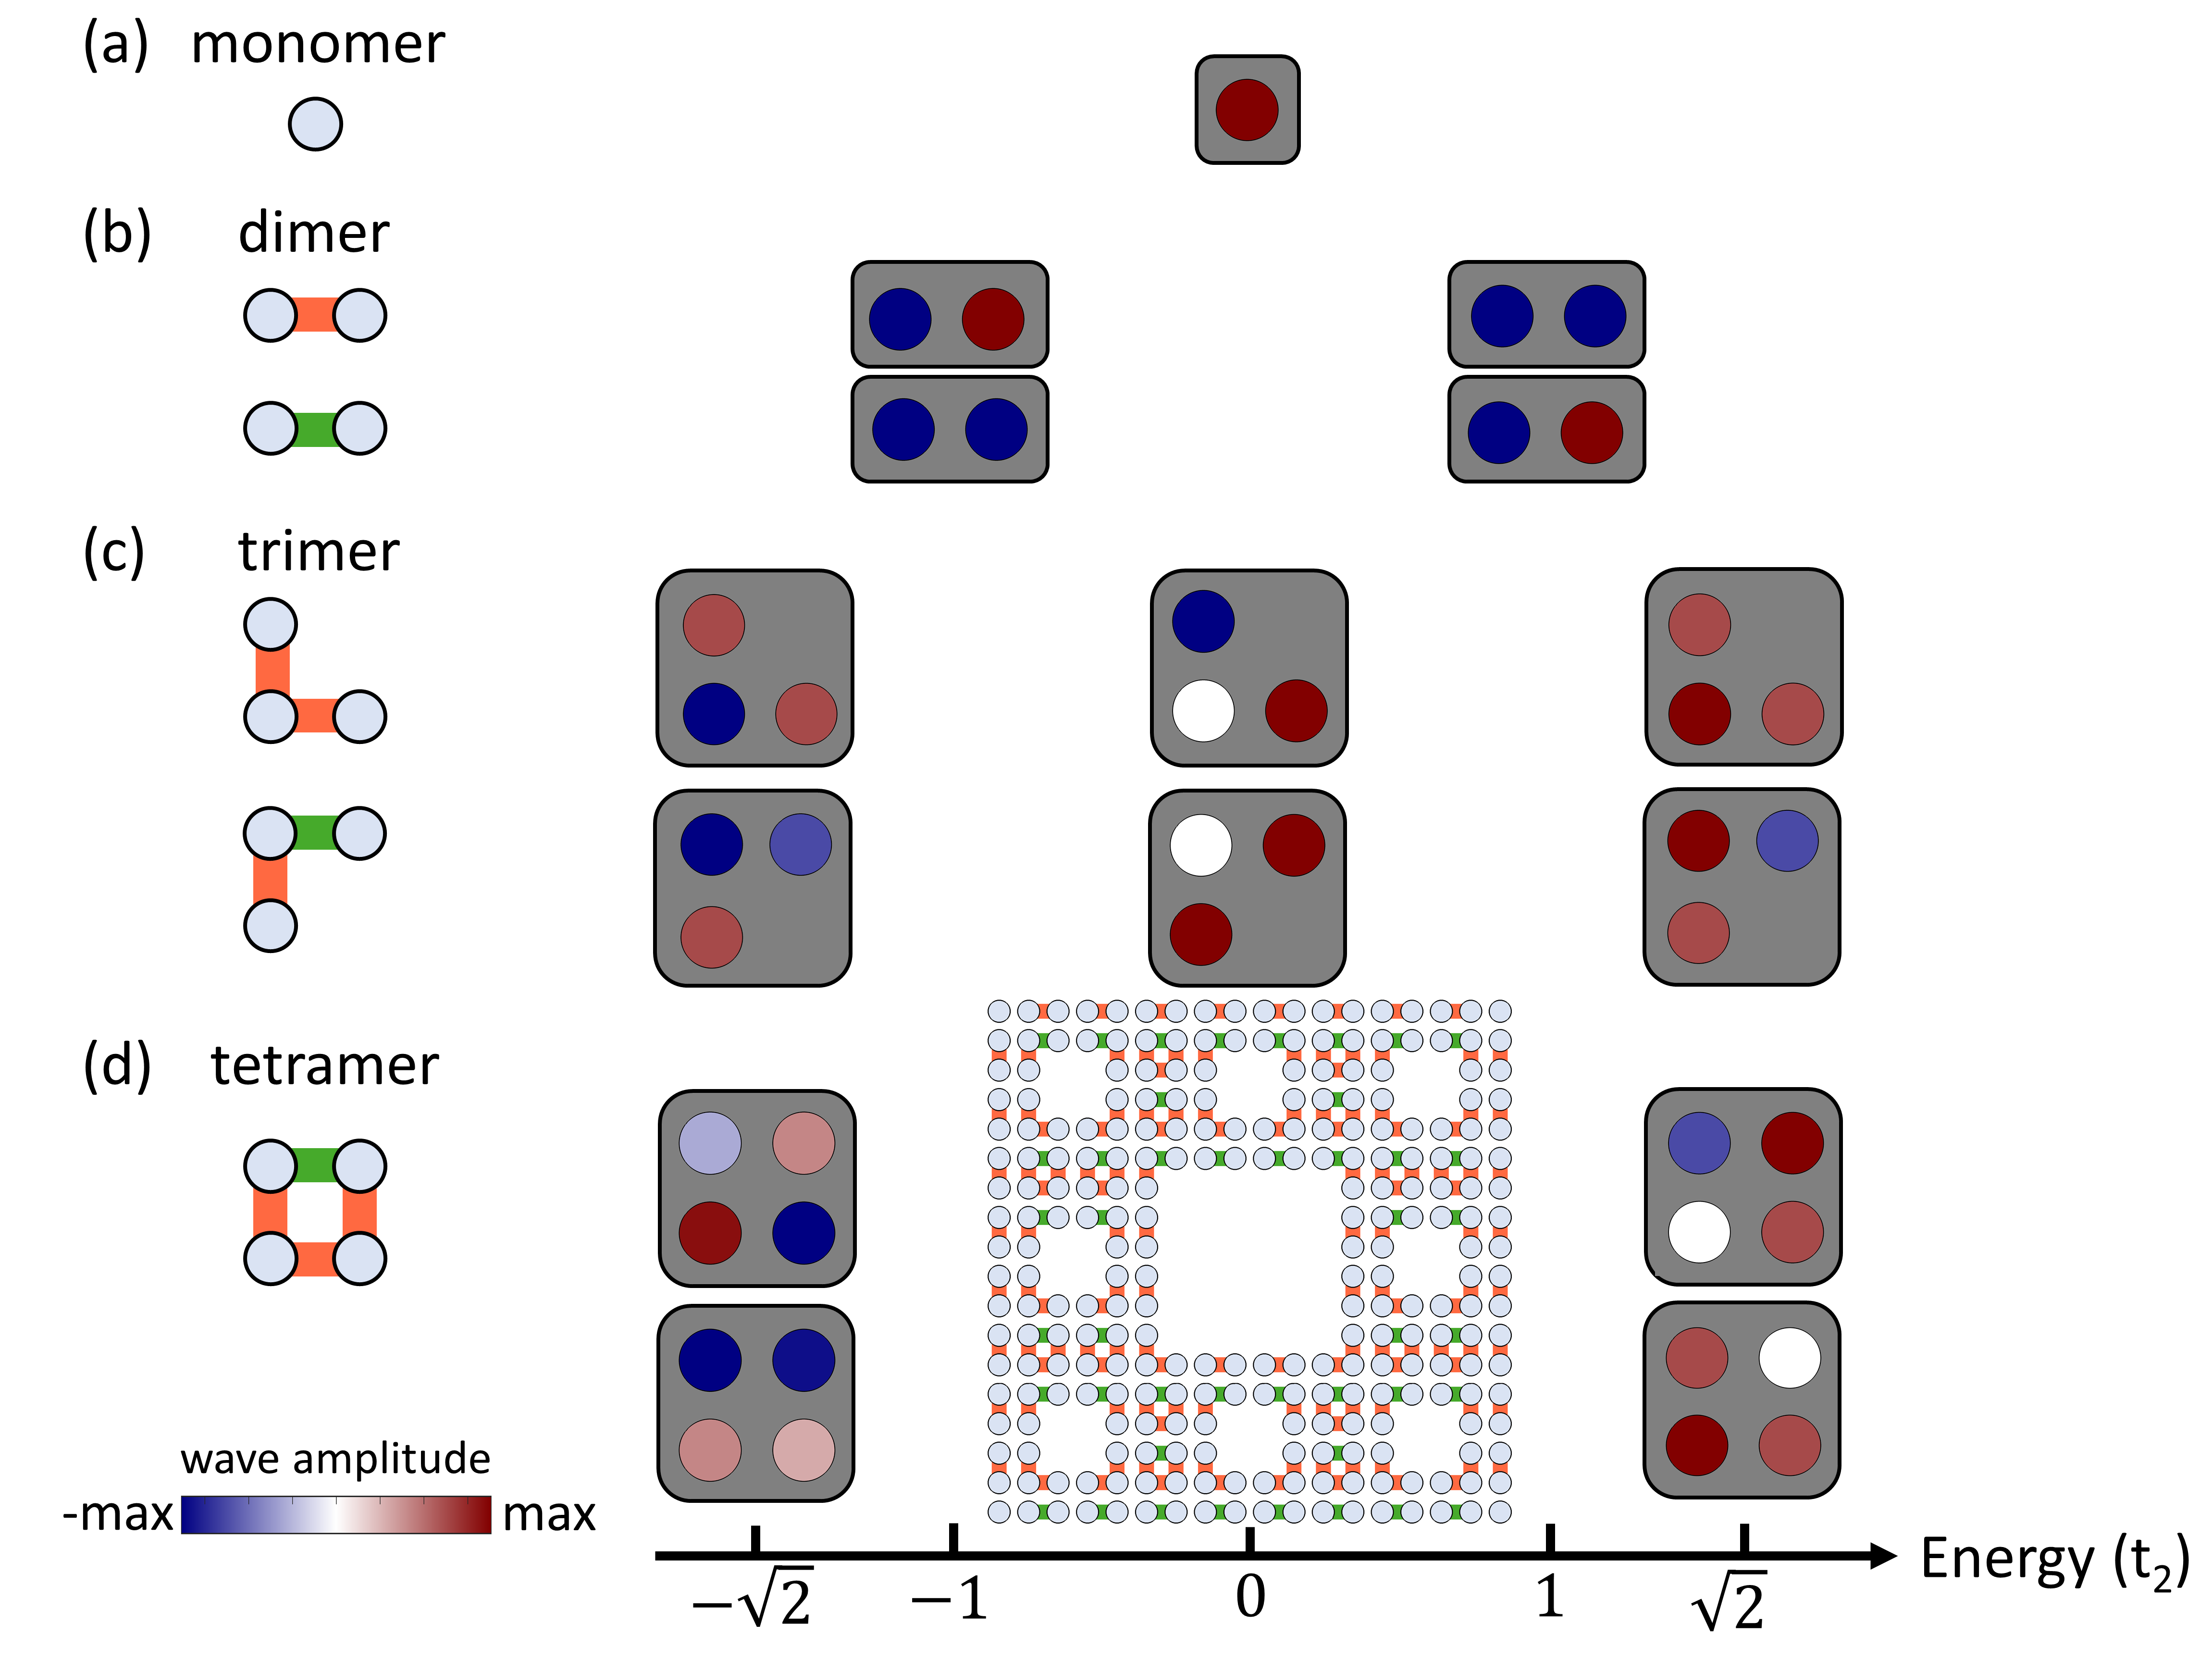
\includegraphics[width=0.75\linewidth]{figure/HOTITheo/Elemen.png}
    \caption{分形晶格中基本单元在 \( t_1=0 \) 时的本征态}(a-d) 分别展示了单体、二聚体、三聚体和四聚体在外角、边缘、内角和“体”区域的本征值与本征向量。红色(绿色)线表示正(负)跃迁。插图:\( t_1=0 \) 时的分形晶格结构。
    \label{fig:Elemen}
\end{figure}

在图\ref{fig:Elemen}(a)中,我们描绘了能量为零的单体的本征矢,其对应于外部角态。二聚体则出现于边缘态,如图\ref{fig:Elemen}(b)所示。由于其同时支持键合态和反键合态,两个二聚体的本征矢可以相互交换。类似地,在图\ref{fig:Elemen}(c)中,三聚体也具有两种不同类型的空间分布,并且可以表现出不同的内部角态,其本征值为$±t_2$和0。 本征值为$E=±t_2$的内角态是对称本征态,而本征值为$E=0$内角态是反对称态。我们还在图\ref{fig:Elemen}(d)中展示了四聚体的本征值和本征矢,它们贡献于“体态”。需要注意的是,由于四聚体和三聚体的本征值都分布在$E=±\sqrt{2}t_2$处,基于三聚体的内部角态在$t_1$有限时与“体态”混合,无法直接观察到。

首先,我们设定 \( t_1/t_2=0.13 \) 并在图\ref{fig:MixElem}(a) 中展示其能谱。接着,我们在图\ref{fig:MixElem}(b) 中绘制状态编号 68 的空间分布。需要注意的是,我们只能找到一个混合态,其概率分布同时出现在内角和“体”区域,而不像图\ref{fig:Elemen}中分别呈现的三聚体与四聚体模式。此外,我们在图\ref{fig:MixElem}(c) 中展示了“体”态的总分布。这些结果表明,在我们的分形模型中,三聚体与四聚体模式发生混合,无法被单独区分。

\begin{figure}[htbp]
    \centering
    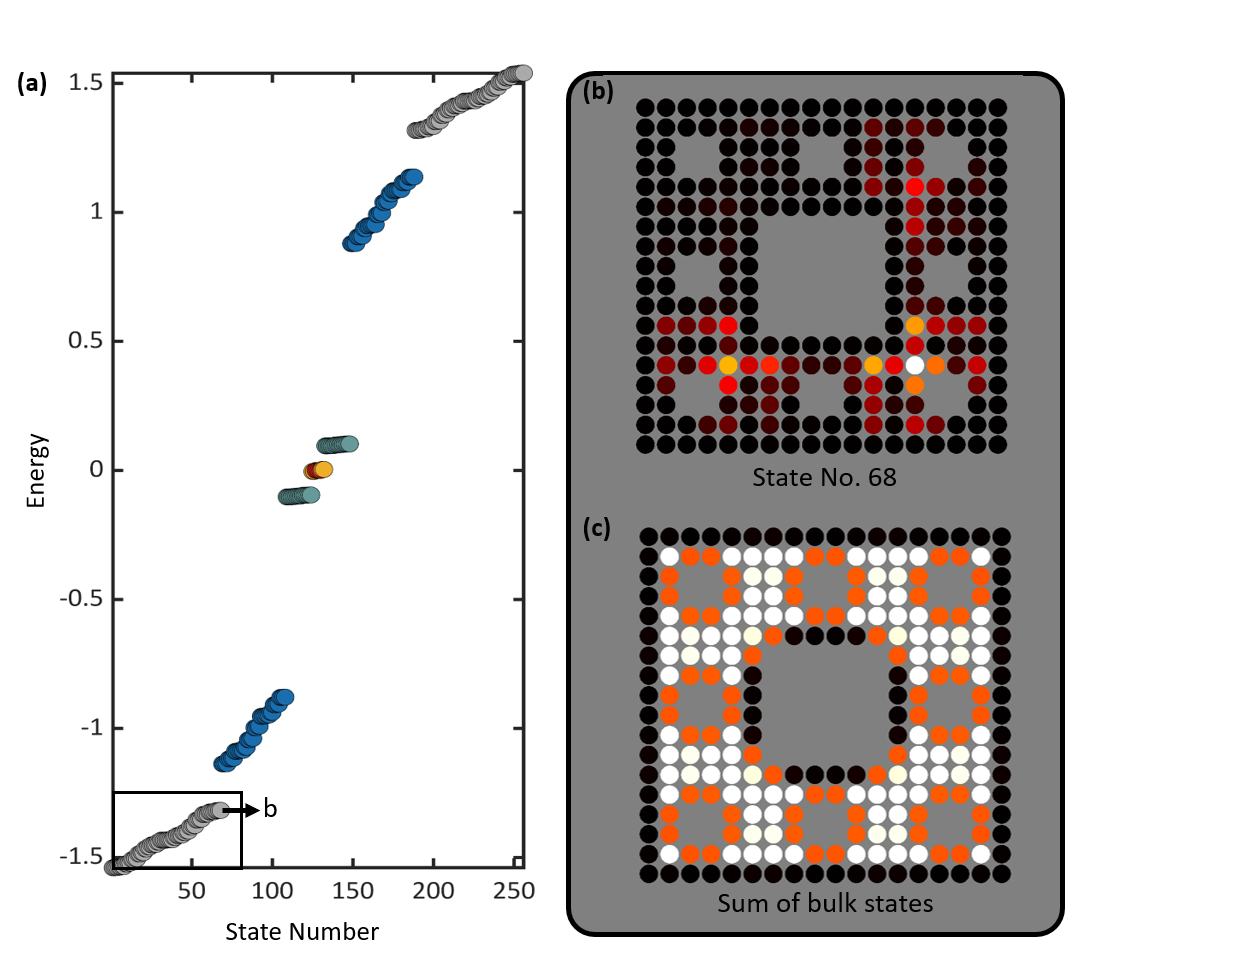
\includegraphics[width=0.6\linewidth]{figure/HOTITheo/MixElem.png}
    \caption{在 \( t_1 \neq 0 \) 时三聚体与四聚体模式的混合}(a) 当 \( t_1/t_2=0.13 \) 时的能谱。(b) 状态编号 68 的空间分布,对应于 (a) 中黑色箭头指示的状态。(c) “体”态的总分布,对应于 (a) 中黑色框内的灰色点。
    \label{fig:MixElem}
\end{figure}

\subsection{G(3)晶格的能谱与拓扑态}
在前文中,我们采用 G(2) 分形晶格进行研究。在此,图\ref{fig:G2Spec}(a) 显示了 G(3) 晶格的能谱及其场分布,作为站点内跃迁 \( t_1 \) 的函数,表明存在更复杂的分形“蝴蝶”结构。

\begin{figure}[htbp]
    \centering
    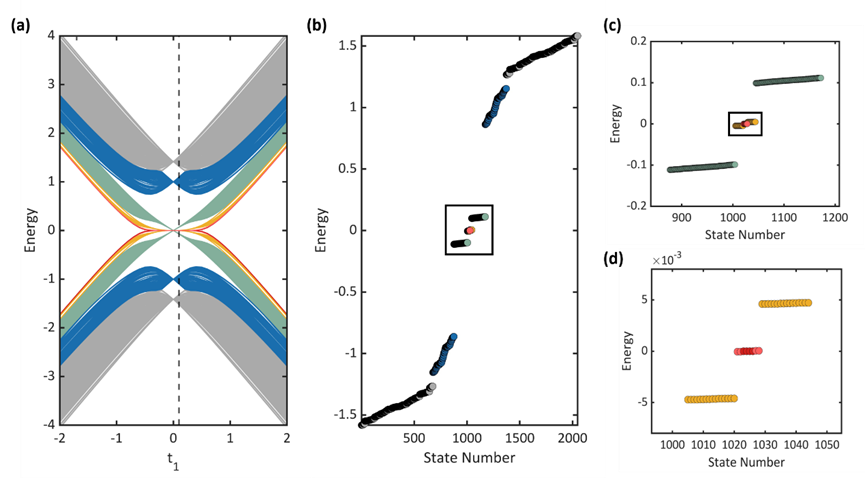
\includegraphics[width=0.75\linewidth]{figure/HOTITheo/G2Spec.png}
    \caption{G(3) 晶格的能谱}(a) 能谱作为站点内跃迁 \( t_1 \) 的函数。红色、粉色、黄色和绿色线分别表示外角态、内角态 A、内角态 B 和内角态 C。蓝色(灰色)线分别表示边缘态(“体”态)。(b-d) 在 \( t_1=0.1 \) 时的能谱。
    \label{fig:G2Spec}
\end{figure}

为了进一步研究态的自相似性,我们在图\ref{fig:G2Spec}(b-d) 中绘制了当 \( t_1=0.1 \) 时的能谱(该值由 (a) 中的黑色虚线标记)。其中,(c) 是 (b) 中黑色框的放大视图,而 (d) 是 (c) 中黑色框的进一步放大视图。在 (d) 中,红色和粉色点表示外角态和内角态 A。内角态 B(黄色点)的数量是内角态 A 的 8 倍,并可分裂为分布于内角态 A 两侧的两个对称分支。类似的现象也发生在内角态 C(绿色点)上,其数量是内角态 B 的 8 倍。

上述现象表明,该能谱具有自相似性,并且随着晶格迭代次数的增加,将出现越来越多的自相似态。

随后,我们在图\ref{fig:G2Field}中绘制了外角态与内角态 A、B、C 的总空间分布。不同迭代产生的内角态的空间分布显示出自相似性的特性。

\begin{figure}[htbp]
    \centering
    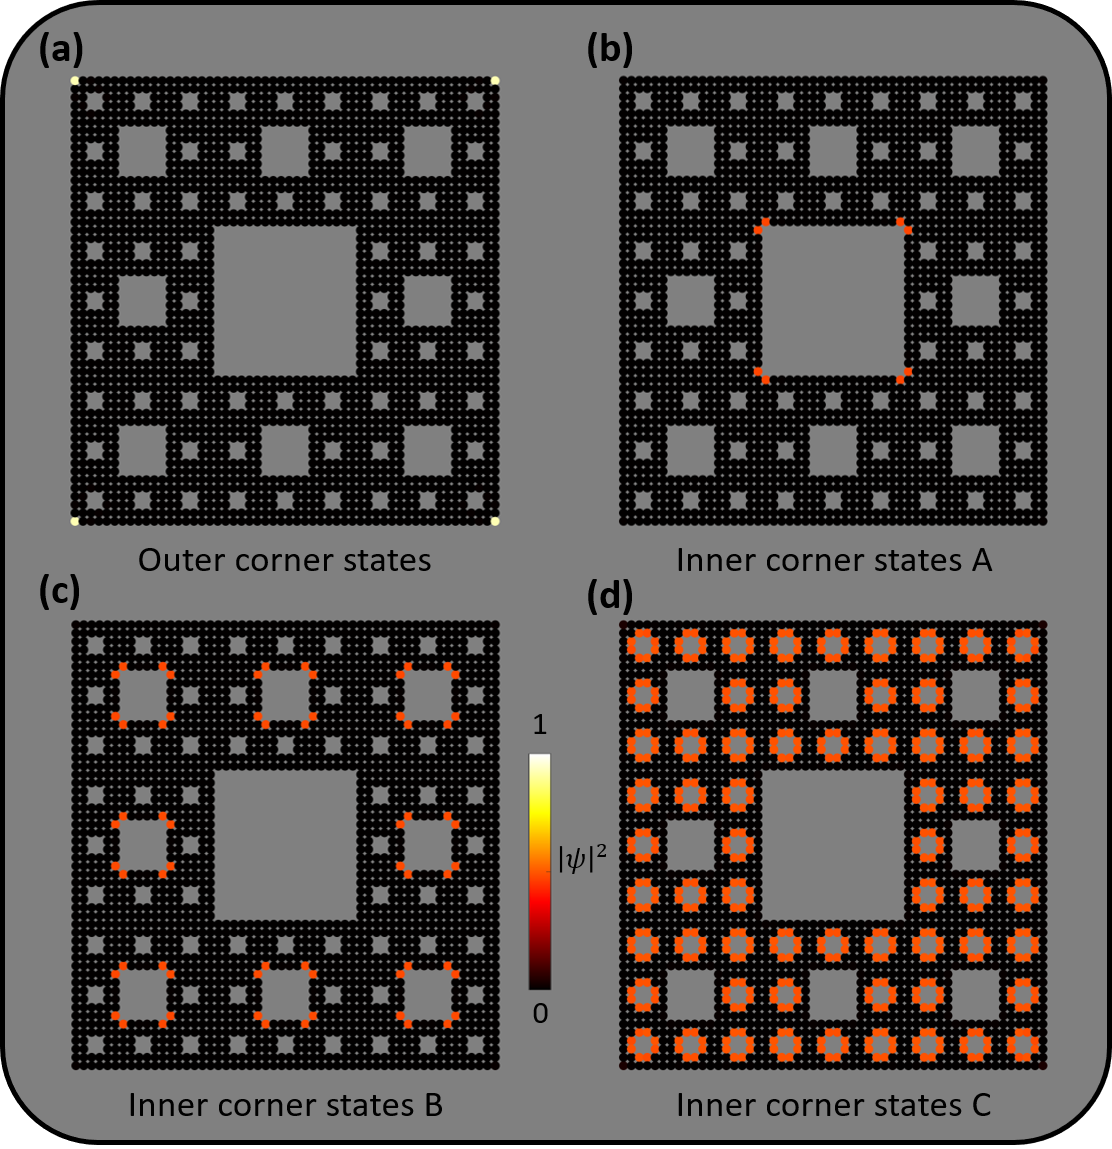
\includegraphics[width=0.5\linewidth]{figure/HOTITheo/G2Field.png}
    \caption{G(3)晶格拓扑态}外角态与标记为 A、B、C 的内角态的总空间分布。
    \label{fig:G2Field}
\end{figure}

\subsection{二维晶格能谱}
作为对比,我们计算了二维方形晶格的BBH模型结果。有限尺寸的方形晶格示意图如图\ref{fig:HOTISpec}(a)所示。计算得到的能量谱随$t_1$的变化如图\ref{fig:HOTISpec}(b, c)所示。其中(b)中晶格尺寸为$L=9$,其与G(2)晶格同尺寸,(c)中晶格尺寸为$L=27$,其与G(3)晶格同尺寸。与分形晶格不同,二维晶格的能量间隙中仅存在四个角态(红线)。
\begin{figure}[htbp]
    \centering
    \includegraphics[width=0.75\linewidth]{figure/HOTITheo/2DSpec.png}
    \caption{方形晶格中的能谱}(a) 方形晶格的示意图。(b, c) 能量谱随内部跳跃$t_1$的变化。(b) $L=9$, (c) $L=27$。
    \label{fig:2DSpec}
\end{figure}

\subsection{拓扑鲁棒性}
为了研究拓扑态的稳健性,我们计算了二维晶格和分形晶格(均处于高阶拓扑相)中拓扑不变量和能谱随无序强度$ 2\sigma $的变化关系。无序按照高斯分布分布,其标准差为 $ \sigma $。

首先,我们在 $ y $ 方向的站点内跃迁中引入手性无序(即相关无序),这一方法已在先前研究中被采用\cite{li2020topological}。如图\ref{fig:Disorder}(a, b) 所示,对于二维方形晶格,经过 1000 次无序实现后的平均四极矩在无序强度 \( 2\sigma = 1.3 \) 处开始下降。而对于分形晶格,平均四极矩的下降发生得更早。因此,如图\ref{fig:Disorder}(c, d) 所示,分形晶格中的角态更早地与“体”态混合,这表明分形晶格中高阶角态的拓扑保护强度较弱。

\begin{figure}[htbp]
    \centering
    \includegraphics[width=1\linewidth]{figure/HOTITheo/Disorder.png}
    \caption{拓扑鲁棒性}(a, b) 方形晶格 (a, c) 和分形晶格 (b, d) 中的四极矩与能谱随手性无序强度的变化关系。手性无序被引入到$y$方向的站点内跃迁中。(e, f) 方形晶格 (e) 和分形晶格 (f) 中的能谱随非手性无序强度的变化关系。非手性无序被添加到现场势中。(g, h) 在 (e, f) 中黑色虚线标记的无序强度下,角局域态的场分布。(c, e) 中的红色点表示四个角局域态。(d, f) 中的黄色和红色点分别表示外角态和内角态。所有结果均基于 1000 次无序实现的平均值。
    \label{fig:Disorder}
\end{figure}

此外,我们在体系的现场势中引入随机无序(非手性无序),结果如图\ref{fig:Disorder}(e-h) 所示。在 (e, f) 中可以看到,分形晶格的角态更早地与“体”态混合,这与手性无序的情况一致。接下来,我们对 (e, f) 中用虚线标记的无序强度下的黄色和红色点对应的状态进行求和(1000 次无序实现),并在 (g) 和 (h) 中绘制相应的场分布。明显可见,在二维晶格中仍然存在角局域态,而在分形晶格中仍然可以观察到外角态和内角态,这与无序前的清洁系统类似。因此,在随机无序的情况下,我们得出的结论仍然成立,即拓扑保护仍然存在,但分形晶格中角态的稳健性弱于二维晶格中的角态。需要注意的是,由于缺乏手性对称性,此前采用的四极矩不变量不再是一个良好的量子化数\cite{li2020topological}。

总体而言,我们得出结论:我们的高阶分形模型是拓扑受保护的,但其保护强度弱于方形晶格。

\section{晶格与拓扑态和维度}
在分形维度模型中呈现出令人着迷的状态后,我们进一步研究这些状态的维度。通过盒计数法\cite{Mandelbrot1982},我们使用以下公式计算晶格、角态和边缘态的维度:
\begin{equation}
D = \lim_{n \to \infty} \frac{\ln (N)}{\ln (N_l)}
\label{eq:BoxCounting}
\end{equation}
其中,\( N \) 表示晶格站点或拓扑态的数量,\( N_l \) 表示单边的站点数。对于每一次迭代生成,相应的盒数如表\ref{tab:Generation}所示。在图\ref{fig:Dimension}中,我们绘制了不同代数 \( G(n) \) 下,\( \ln N / \ln N_l \) 随迭代次数变化的曲线,分别对应内角态、外角态、边缘态和整个晶格。

\begin{table}[htbp]
    \centering
    \begin{tabular}{|c|c|c|c|c|}
        \hline
        迭代代数 & G(1) & G(2) & G(3) & G(n) \\
        \hline
        总盒数 \(N_s\) & 32 & 256 & 2048 & \(4 \times 8^n\) \\
        \hline
        横向盒数 \(N_l\) & 6 & 18 & 54 & \(2 \times 3^n\) \\
        \hline
        外角态盒数 \(N_o\) & 4 & 4 & 4 & 4 \\
        \hline
        内角态盒数 \(N_i\) & 8 & 72 & 584 & \(\sum_{i=1}^{n} 8^i\) \\
        \hline
        边缘态盒数 \(N_e\) & 16 & 80 & 400 & \(8 \times (3^n - 1) + \sum_{i=1}^{n-1} (3^i - 1) \times 8^{n-i}\) \\
        \hline
    \end{tabular}
    \caption{分形晶格每次迭代所对应的盒数}在每次迭代中,总盒数 \( N_s \) 包括所有覆盖 Sierpinski 地毯的盒子,而横向盒数 \( N_l \) 表示分形晶格单边上的盒子数。盒数 \( N_o \)、\( N_i \) 和 \( N_e \) 分别对应于外角态、内角态和边缘态。
\label{tab:Generation}
\end{table}

\begin{figure}[htbp]
    \centering
    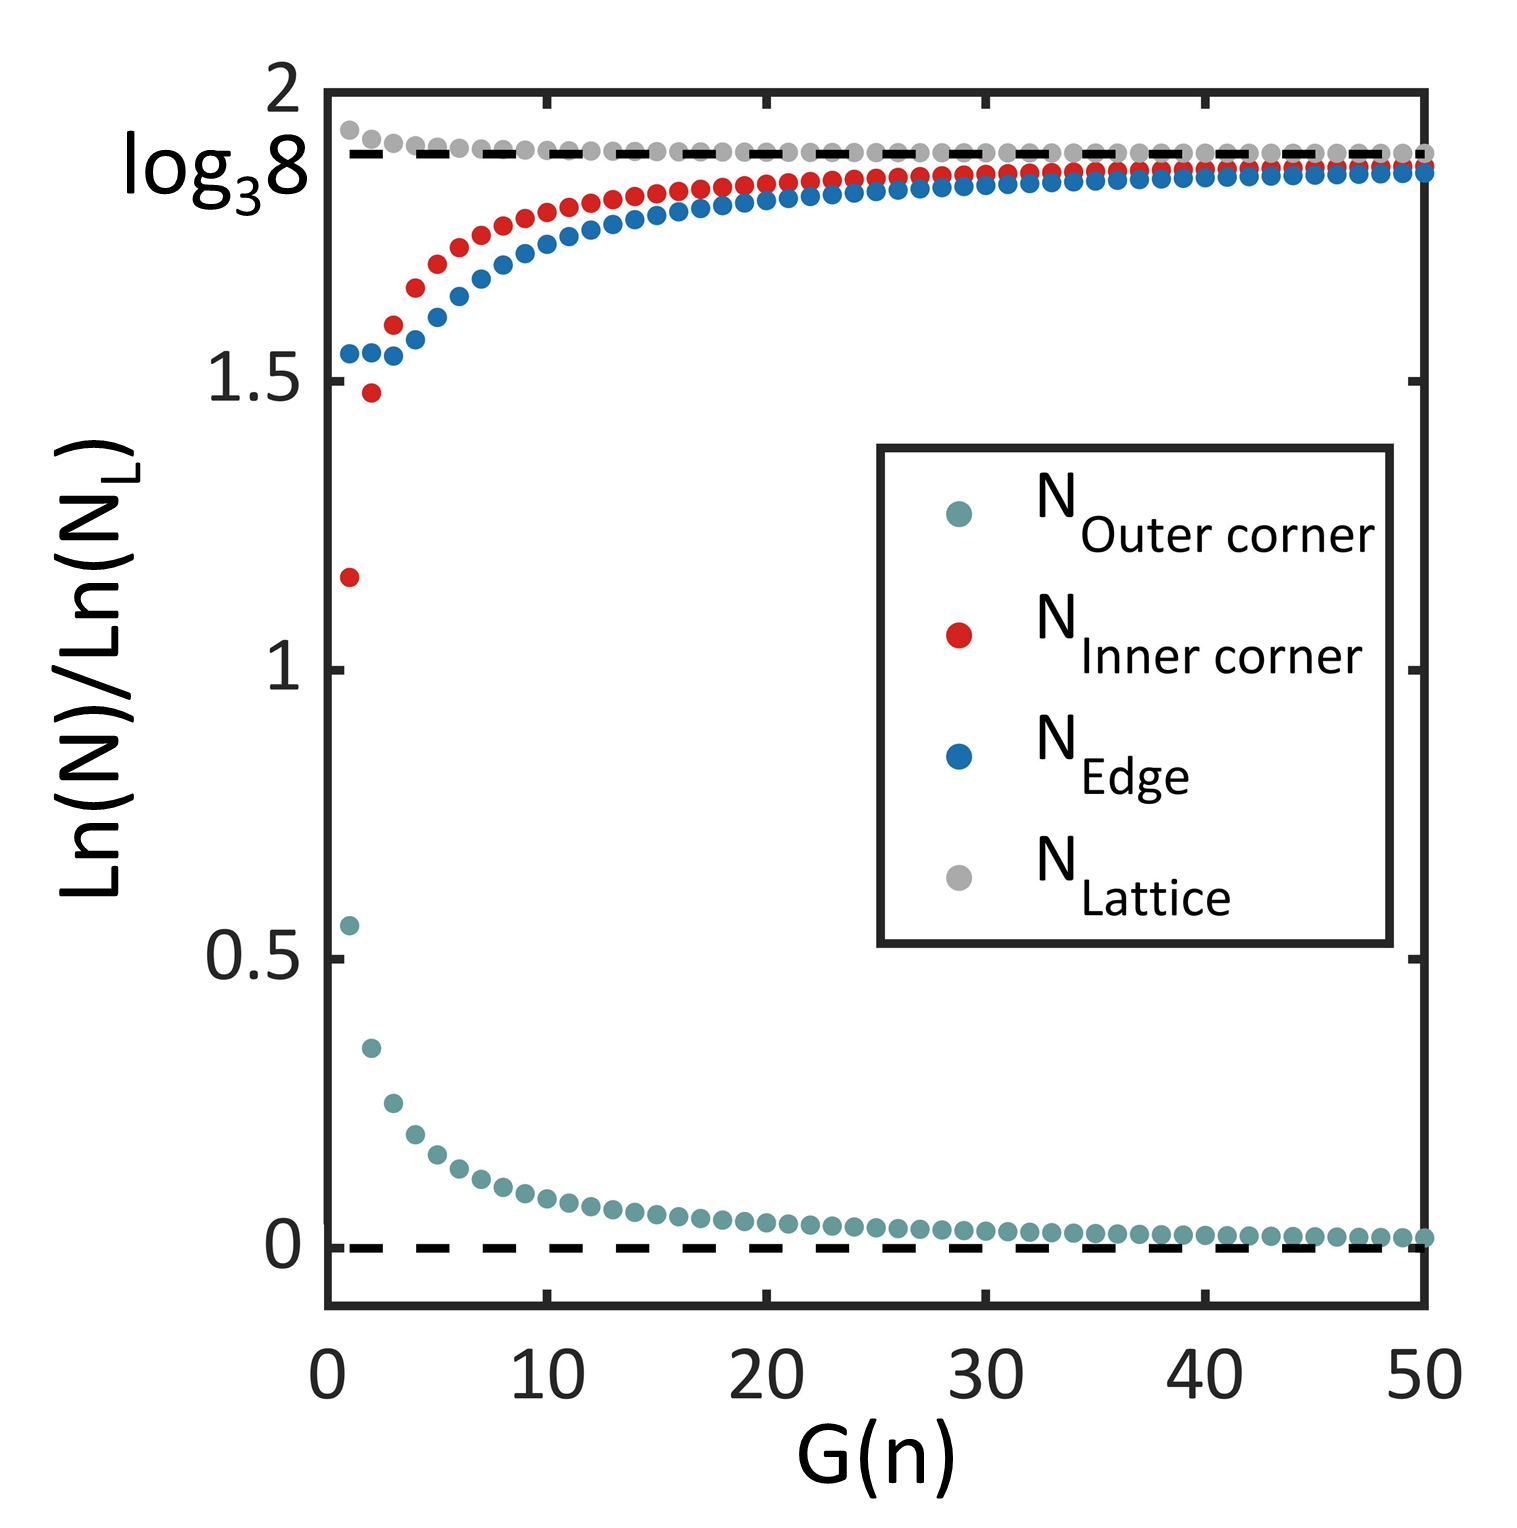
\includegraphics[width=0.5\linewidth]{figure/HOTITheo/Dimension.png}
    \caption{拓扑态维度}外角态、内角态、边缘态及分形晶格的维度随迭代代数的变化关系。
    \label{fig:Dimension}
\end{figure}

为了计算分形晶格、角态和边缘态的维度,我们采用盒计数法。将每次迭代的盒数代入公式\ref{eq:BoxCounting}本章采用的谢宾斯基地毯分形晶格的维度$D_s$可以计算为:

\begin{equation}
D_s = \lim_{n \to \infty} \frac{\ln (N_s)}{\ln (N_l)} = \lim_{n \to \infty} \frac{\ln 4 \times 8^n}{\ln 2 \times 3^n} = \frac{\ln 8}{\ln 3} \approx 1.89
\end{equation}
可以看到,在图\ref{fig:Dimension}中,灰色的点对应了晶格的计算结果,随着迭代增加,其逐渐趋于$D=\log_38$的虚线。类似的,我们继续计算外角态的维度$D_{oc}$:
\begin{equation}
D_{oc} = \lim_{n \to \infty} \frac{\ln (N_c)}{\ln (N_l)} = \lim_{n \to \infty} \frac{\ln 4}{\ln 2 \times 3^n} = 0
\end{equation}
可以观察到,在图\ref{fig:Dimension}中,随着代数的增加,外角态的维度$D_{oc}$趋近于 0(绿色点)。结合 1.89 维晶格(灰色点),我们得出余维数为 1.89,因此外角态的结果对应于一个分数阶拓扑绝缘体。

内角态$D_{ic}$和边缘态$D_e$的结果则与外角态非常不同:
\begin{equation}
D_{ic}= \lim_{n \to \infty} \frac{\ln (N_c)}{\ln (N_l)} = \lim_{n \to \infty} \frac{\ln \sum_{i=1}^{n} 8^i}{\ln 2 \times 3^n} = \frac{\ln 8}{\ln 3} \approx 1.89
\end{equation}

\begin{equation}
D_e = \lim_{n \to \infty} \frac{\ln (N_e)}{\ln (N_l)} = \lim_{n \to \infty} \frac{\ln 8 \times (3^n - 1) + \sum_{i=1}^{n-1} (3^i - 1) \times 8^{n-i}}{\ln 2 \times 3^n} = \frac{\ln 8}{\ln 3} \approx 1.89
\end{equation}
令人惊讶的是,内角态维度$D_{ic}$和边缘态维度$D_e$均为 1.89,与晶格维度一致。这意味其对应的余维数为 0。在分形晶格中,内角态和边缘态的数量随着系统尺寸呈指数级增长。这些反直觉的结果此前从未被报道,表明分形模型中的高阶拓扑绝缘体与传统的高阶拓扑绝缘体存在显著差异。

此外,我们可以计算在无限迭代(\( n \to \infty \))下,内角态、边缘态和“体”态的比例,如下所示:
\begin{equation}
r_{\text{inner corner}} = \lim_{n \to \infty} \frac{N_i}{N_s} = \lim_{n \to \infty} \frac{\sum_{i=1}^{n} 8^i}{4 \times 8^n} = \frac{2}{7}
\end{equation}

\begin{equation}
r_{\text{edge}} = \lim_{n \to \infty} \frac{N_e}{N_s} = \lim_{n \to \infty} \frac{8 \times (3^n - 1) + \sum_{i=1}^{n-1} (3^i - 1) \times 8^{n-i}}{4 \times 8^n} = \frac{4}{35}
\end{equation}

\begin{equation}
r_{\text{bulk}} = 1 - r_{\text{inner corner}} - r_{\text{edge}} = \frac{3}{5}
\end{equation}

\section{压缩的拓扑相图}
\subsection{分形晶格的拓扑相图}
如图\ref{fig:Quadrupole}所示,我们系统研究了四极矩序参量$Q_{xy}$在分形晶格(红色数据点)与常规二维方晶格(灰色数据点)中随胞内跳跃参数$t_1$的演化规律。值得注意的是,分形晶格体系展现出独特的拓扑响应特征:当$t_1$跨越临界值$\pm 0.35$时,$Q_{xy}$发生量子化跃迁,从零值突变为$0.5$,并在区间$-0.35 < t_1 < 0.35$内保持稳定的平台值。这与传统二维体系(灰色虚线)的连续渐变行为形成鲜明对比,证实分形几何导致拓扑非平庸区域发生显著压缩,该现象可能与Hausdorff维度($d_h \approx 1.89$)引起的量子限域效应密切相关。

\begin{figure}[htbp]
    \centering
    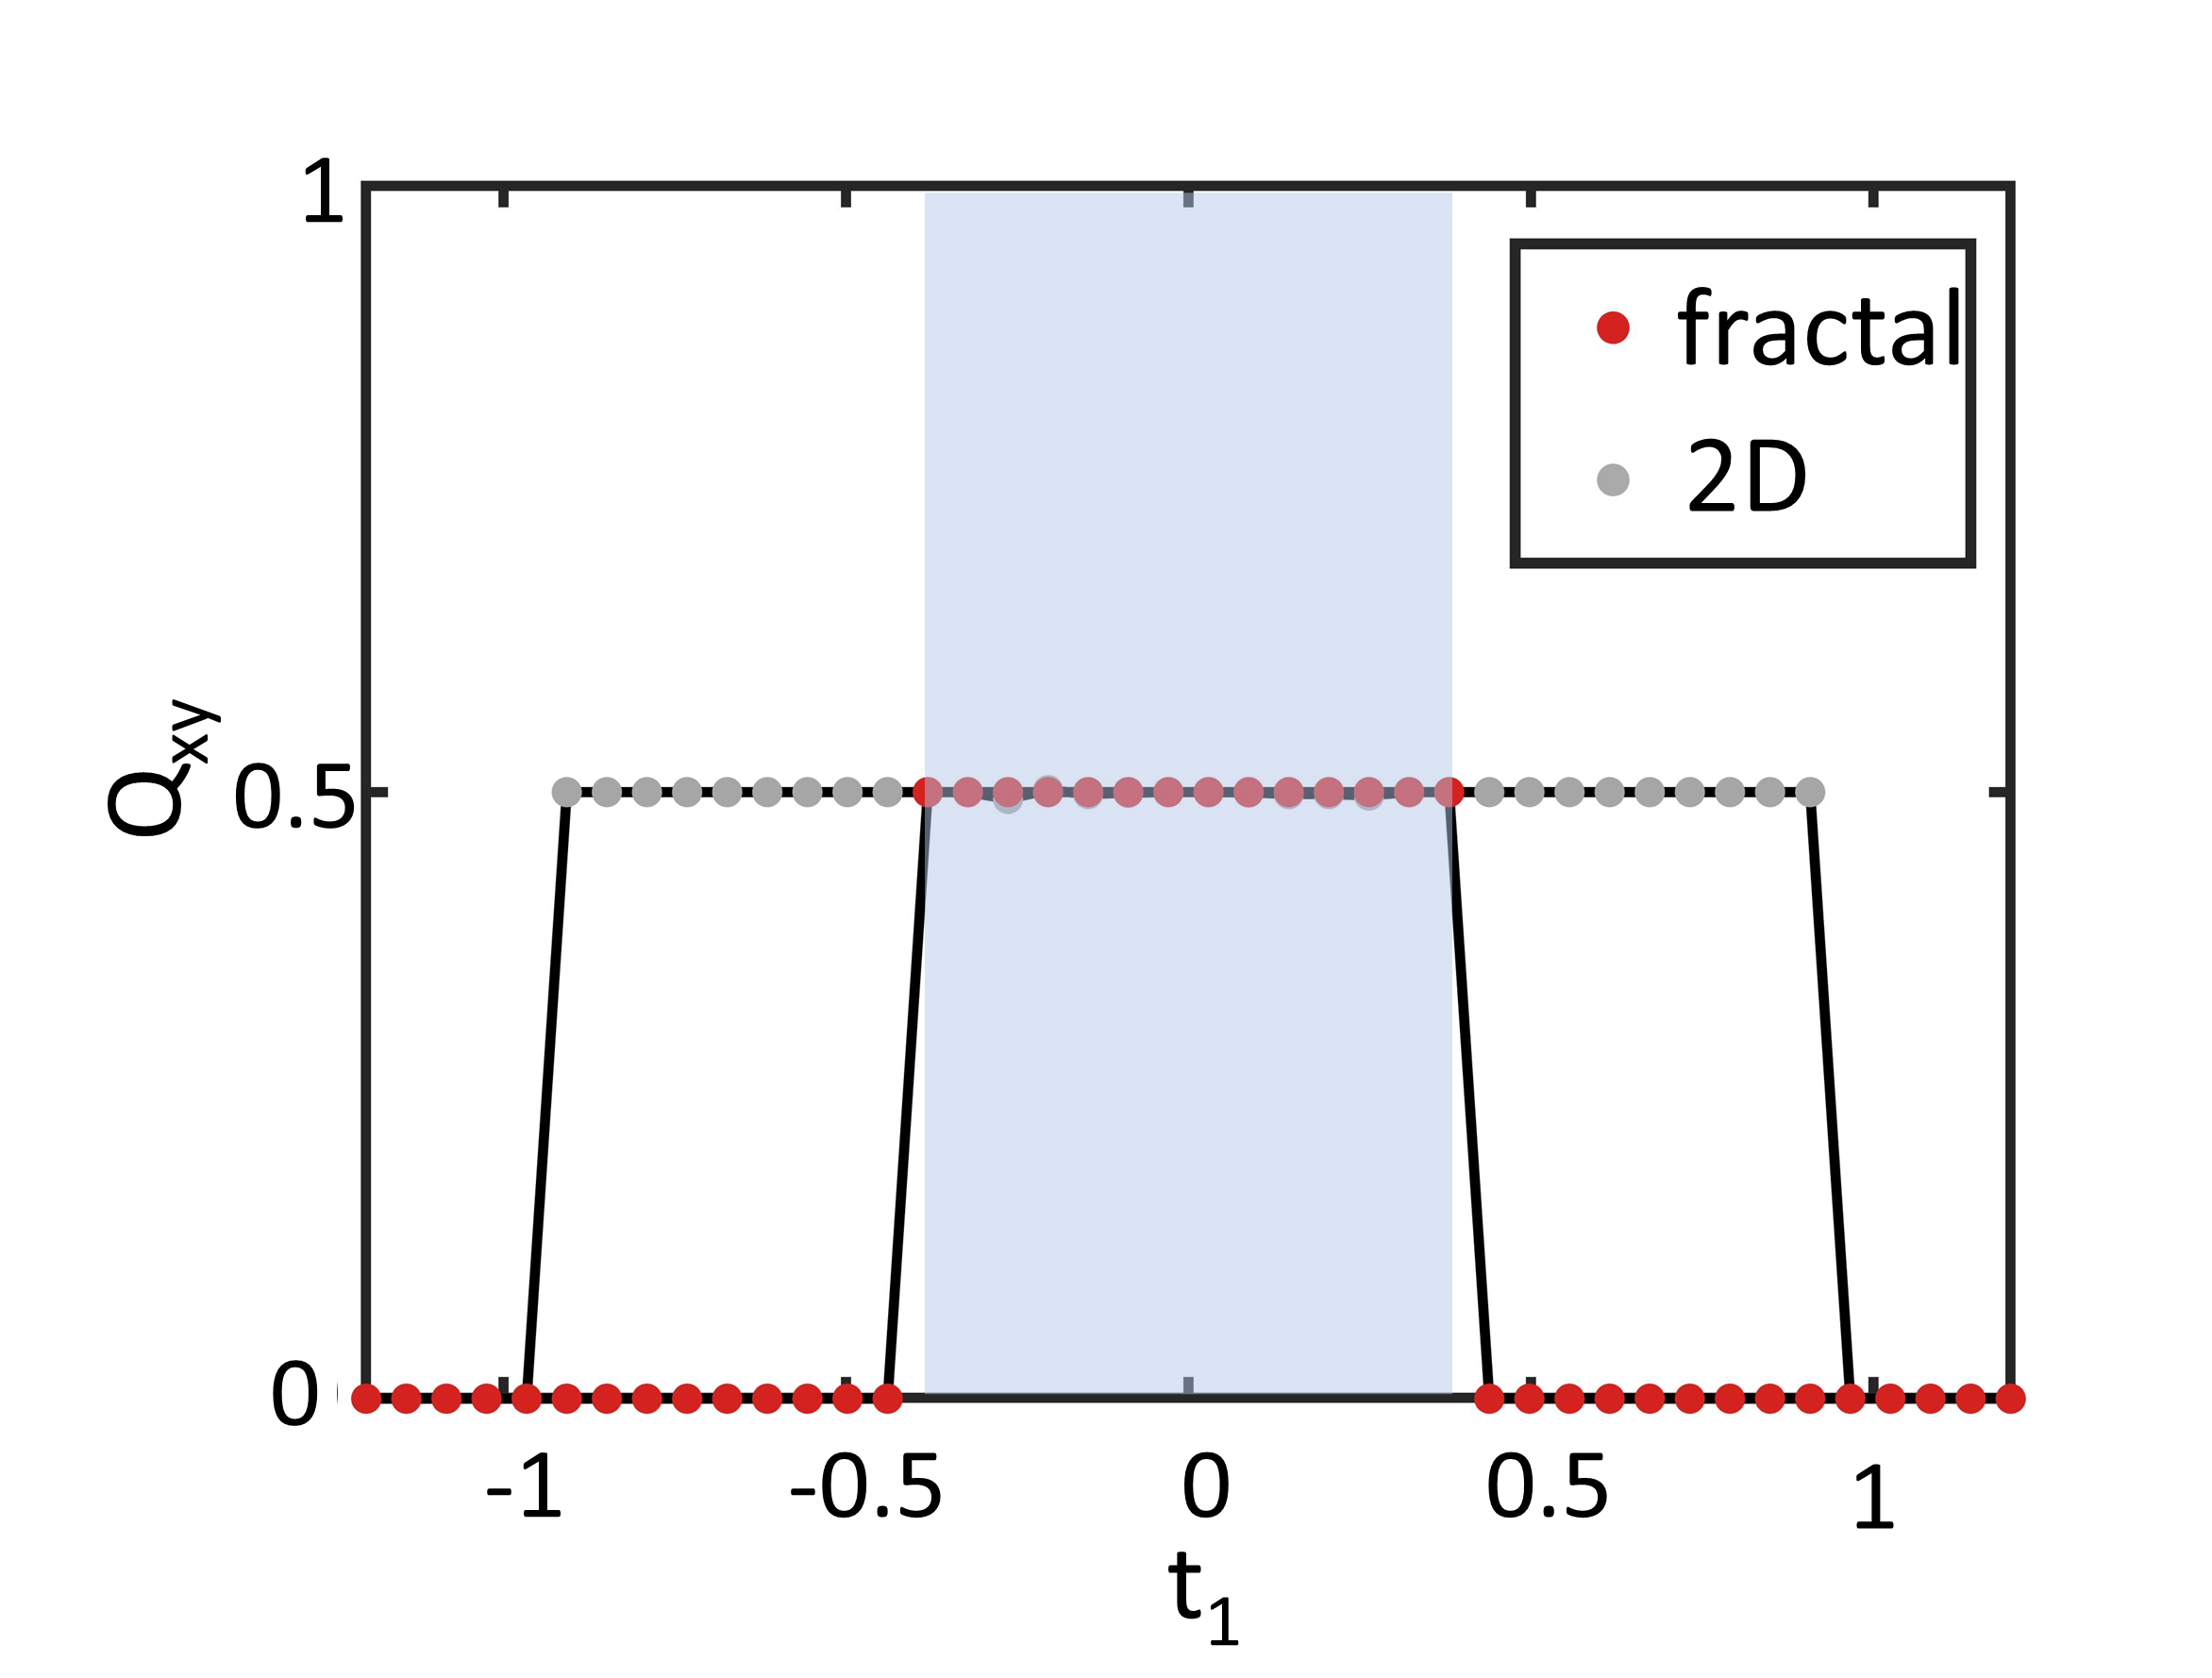
\includegraphics[width=0.5\linewidth]{figure/HOTITheo/Quadrupole.png}
    \caption{压缩的拓扑相图}灰色与红色点代表2维晶格和分形晶格的四极矩。蓝色区域标记为分形晶格的拓扑区域。
    \label{fig:Quadrupole}
\end{figure}

为深入揭示维度对拓扑物态的影响机制,我们选取三个特征参数比进行本征态场分布研究:
\begin{itemize}
    \item [$(i)$] $t_1/t_2=0.1$(二维与1.89维体系均处于拓扑非平庸相)
    \item [$(ii)$] $t_1/t_2=0.8$(二维体系保持非平庸而分形晶格退化为平庸相)
    \item [$(iii)$] $t_1/t_2=1.1236$(即$t_2/t_1=0.89$,两种体系均处于平庸相)
\end{itemize}

\begin{figure}[htbp]
    \centering
    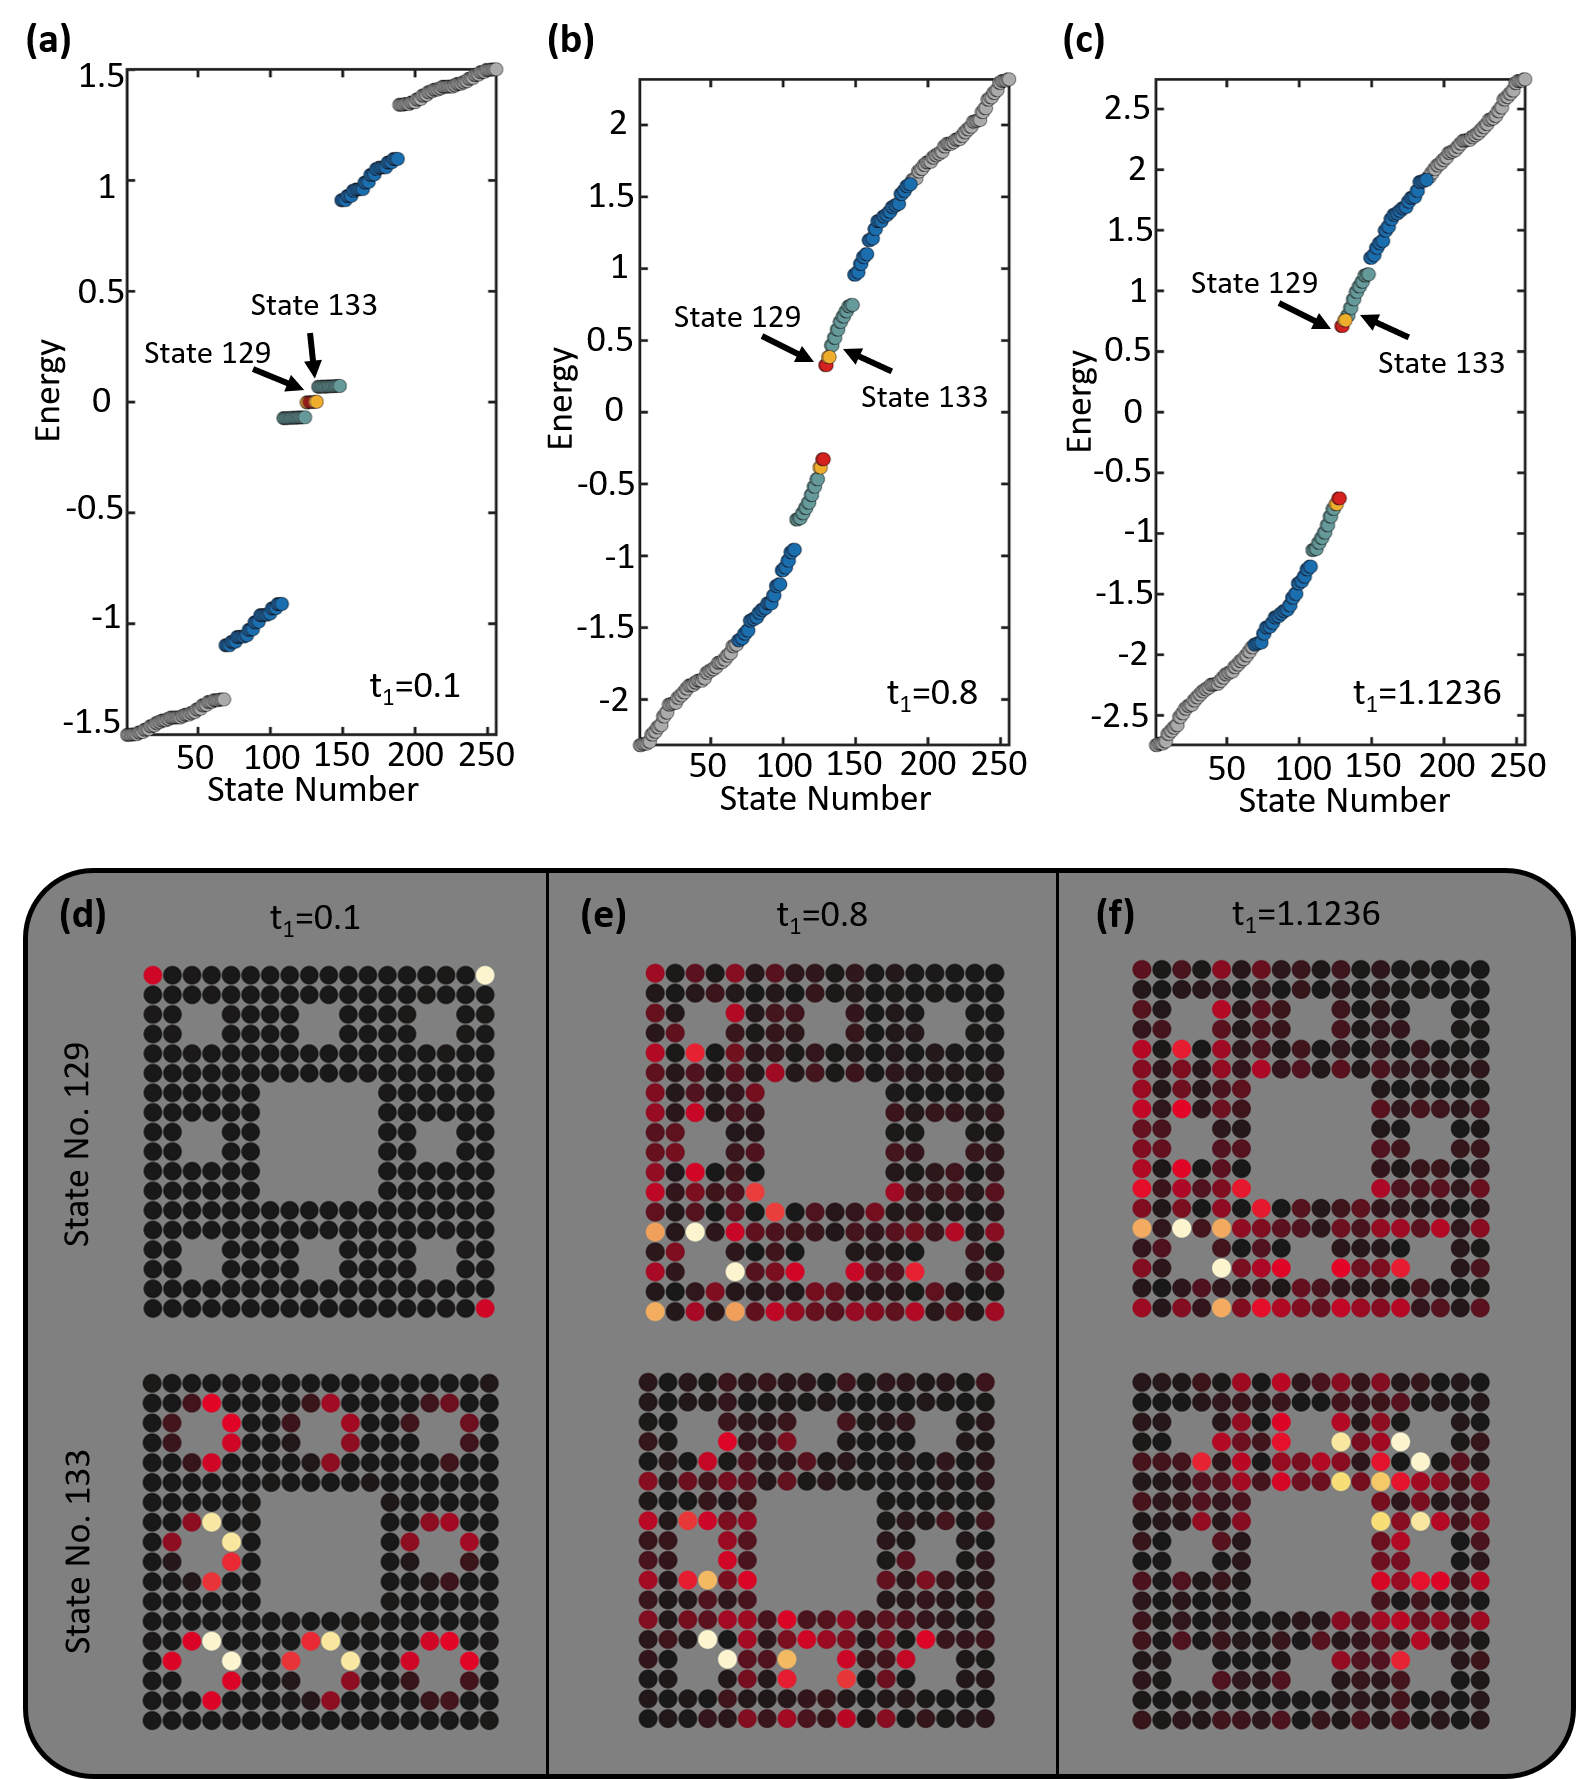
\includegraphics[width=0.75\linewidth]{figure/HOTITheo/Transition.png}
    \caption{分形晶格中的非平庸态与平庸态}(a-c) 分别为$t_1/t_2=0.1$、$t_1/t_2=0.8$和$t_1/t_2=1.1236$时的能量谱。(d-f) 在$t_1/t_2=0.1$、$t_1/t_2=0.8$和$t_1/t_2=1.1236$时,第129号和第133号态的场分布。晶格间跳跃$t_2$设为1。
    \label{fig:Transition}
\end{figure}

通过精确对角化计算获得的分形晶格能谱如图\ref{fig:Transition}(a-c)所示。在拓扑非平庸情形$(i)$下,体系呈现典型的角态-边缘态-体态能隙分离特征。特别地,第129号本征态(外角态)与第133号本征态(内角态)的空间分布如图\ref{fig:Transition}(d)所示,其波函数显著局域于晶格顶角区域,符合高阶拓扑绝缘体的判断标准。当调节至参数$(ii)$时(图\ref{fig:Transition}(e)),尽管二维方晶格仍保持非平庸特性,分形晶格中角态完全消失,能隙内仅存在扩展的体态,这直接验证了维度降低导致的拓扑相压缩效应。最终在参数$(iii)$对应的平庸相中(图\ref{fig:Transition}(f)),两种晶格体系均表现出全域退局域化的波函数分布,表明系统进入普通绝缘体相。

上述结果表明,当体系维度$d$满足$d < 2$时,传统二维拓扑分类中的体-边对应关系被打破,拓扑相区域被压缩。这种压缩现象表明,维度可能可以作为一个新的参数调控拓扑相变。

\subsection{不同迭代的拓扑相图}

为验证拓扑相图在不同迭代次数下的收敛性和一致性,我们系统计算了第二代($G(2)$)和第三代($G(3)$)分形晶格的拓扑相图。如图\ref{fig:G3Qxy}(c,d)所示,两个迭代次数下的相图展现出高度一致性,这证实了我们的计算结果具有可靠的收敛性。

\begin{figure}[htbp]
    \centering
    \includegraphics[width=0.5\linewidth]{figure/HOTITheo/G3Qxy.png}
    \caption{不同代数分形晶格的拓扑相图}(a, b) 分别为 G(2) 和 G(3) 代的分形晶格。(c, d) 对应于 (a, b) 的实空间拓扑不变量 \( Q_{xy} \) 随站点内跃迁 \( t_1 \) 变化的关系。
    \label{fig:G3Qxy}
\end{figure}

在$t_1/t_2 < 0.35$的参数区间内,$G(2)$和$G(3)$均保持拓扑非平庸相,其四极矩序参量$Q_{xy}$稳定在0.5的量子化平台值。当$t_1/t_2$跨越临界值$\pm 0.35$时,两个迭代次数的体系均发生拓扑相变,$Q_{xy}$突变为零。在中间参数区域$-0.35 < t_1/t_2 < 0.35$内,相边界位置完全重合。

这种迭代无关性表明,分形晶格的拓扑性质主要由其Hausdorff维度($d_h \approx 1.89$)决定,而对具体的微观结构细节(如迭代次数)不敏感。这一发现为分形拓扑物态的理论研究提供了重要指导:在保证体系维度不变的前提下,采用较低迭代次数的分形结构即可反应可靠的拓扑性质,这大大降低了数值计算和实验实现的复杂度。

\subsection{拓扑相压缩的起源}
在我们的分形晶格中,我们发现了一个压缩的非平庸区域$t_1\in[-0.35,0.35]$。这一有趣的拓扑相压缩可最可能的原因是空间平移对称性的破缺。接下来,我们将讨论拓扑相压缩与空间平移对称性的破缺的关联,并尝试为维度与拓扑的相互作用提供新的见解。

首先,我们注意到分形晶格中的空洞导致了空间平移对称性的破缺。我们计算了具有不同空洞代数的晶格的四极矩,如图\ref{fig:Reason}(a-d)所示。我们可以看到,随着空洞数量的增加,拓扑相变出现在$t_1=\pm1.0$(图\ref{fig:Reason}(e))、$t_1=\pm0.80$(图\ref{fig:Reason}(f))、$t_1=\pm0.67$(图\ref{fig:Reason}(g))和$t_1=\pm0.35$(图\ref{fig:Reason}(h))。图(d)中的晶格是Sierpinski地毯,$t_1=0.35$处的相变与我们在正文中的结果非常吻合。因此,我们可以说空间平移对称性破缺是相压缩的一个原因。

\begin{figure}[htbp]
    \centering
    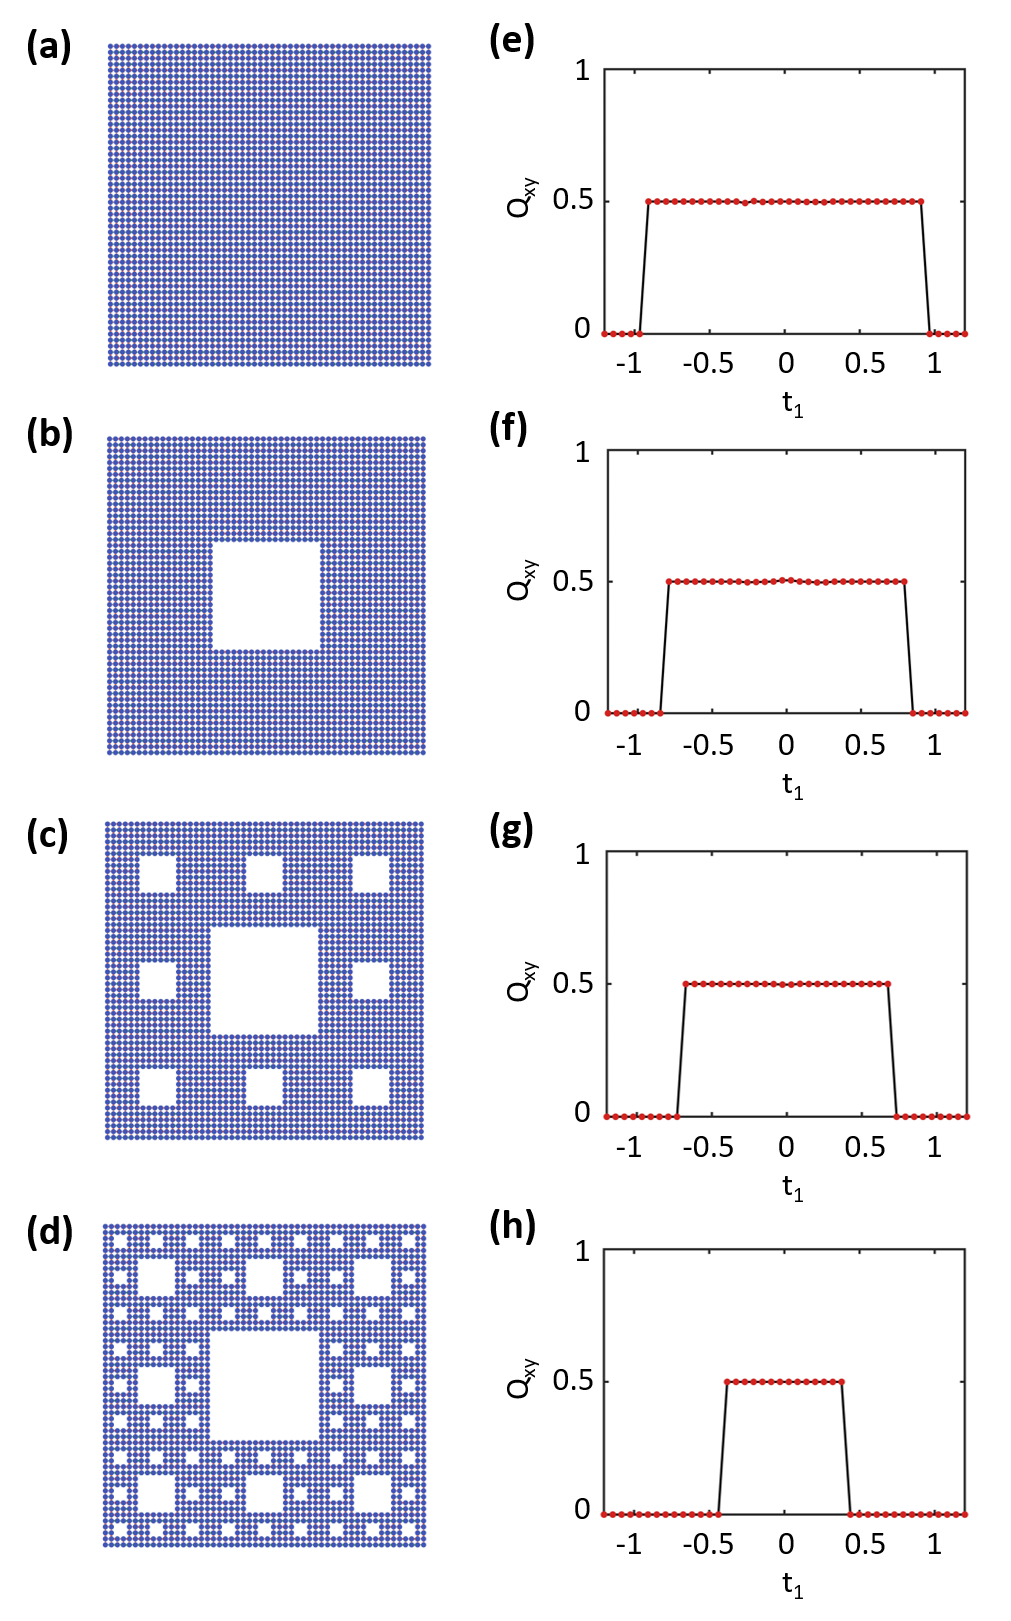
\includegraphics[width=0.5\linewidth]{figure/HOTITheo/Reason.png}
    \caption{具有不同空隙数量的方形晶格的拓扑相图}(a-d) 晶格结构示意图。(e-h) 随着空隙数量增加而收缩的拓扑区域。(d) 对应于第三代 Sierpinski 地毯。
    \label{fig:Reason}
\end{figure}

然而,一个自然的问题出现:如果空隙在二维晶格中是随机分布的会发生什么?为了解决这个问题,我们研究了一个平面方形晶格,并随机移除了 68 个站点。结果表明,该去除部分站点的方形晶格剩余 256 个站点,与 G(2) 代的分形模型站点数相同。

对于特定的实现,我们在 \( t_1 = 0.1 \) 时绘制了能谱,如图\ref{fig:RandDel}(a) 所示。需要注意的是,在分形模型中,不同类型角态之间的能隙消失,并在能量 \( 0 \) 处出现一系列简并态。随后,我们计算了实空间拓扑不变量 \( Q_{xy} \) 随站点内跃迁 \( t_1 \) 变化的关系,并将结果展示在图\ref{fig:RandDel}(b) 中。可以看到,拓扑不变量 \( Q_{xy} \) 不再被量子化,这意味着该系统不是拓扑的。

\begin{figure}[htbp]
    \centering
    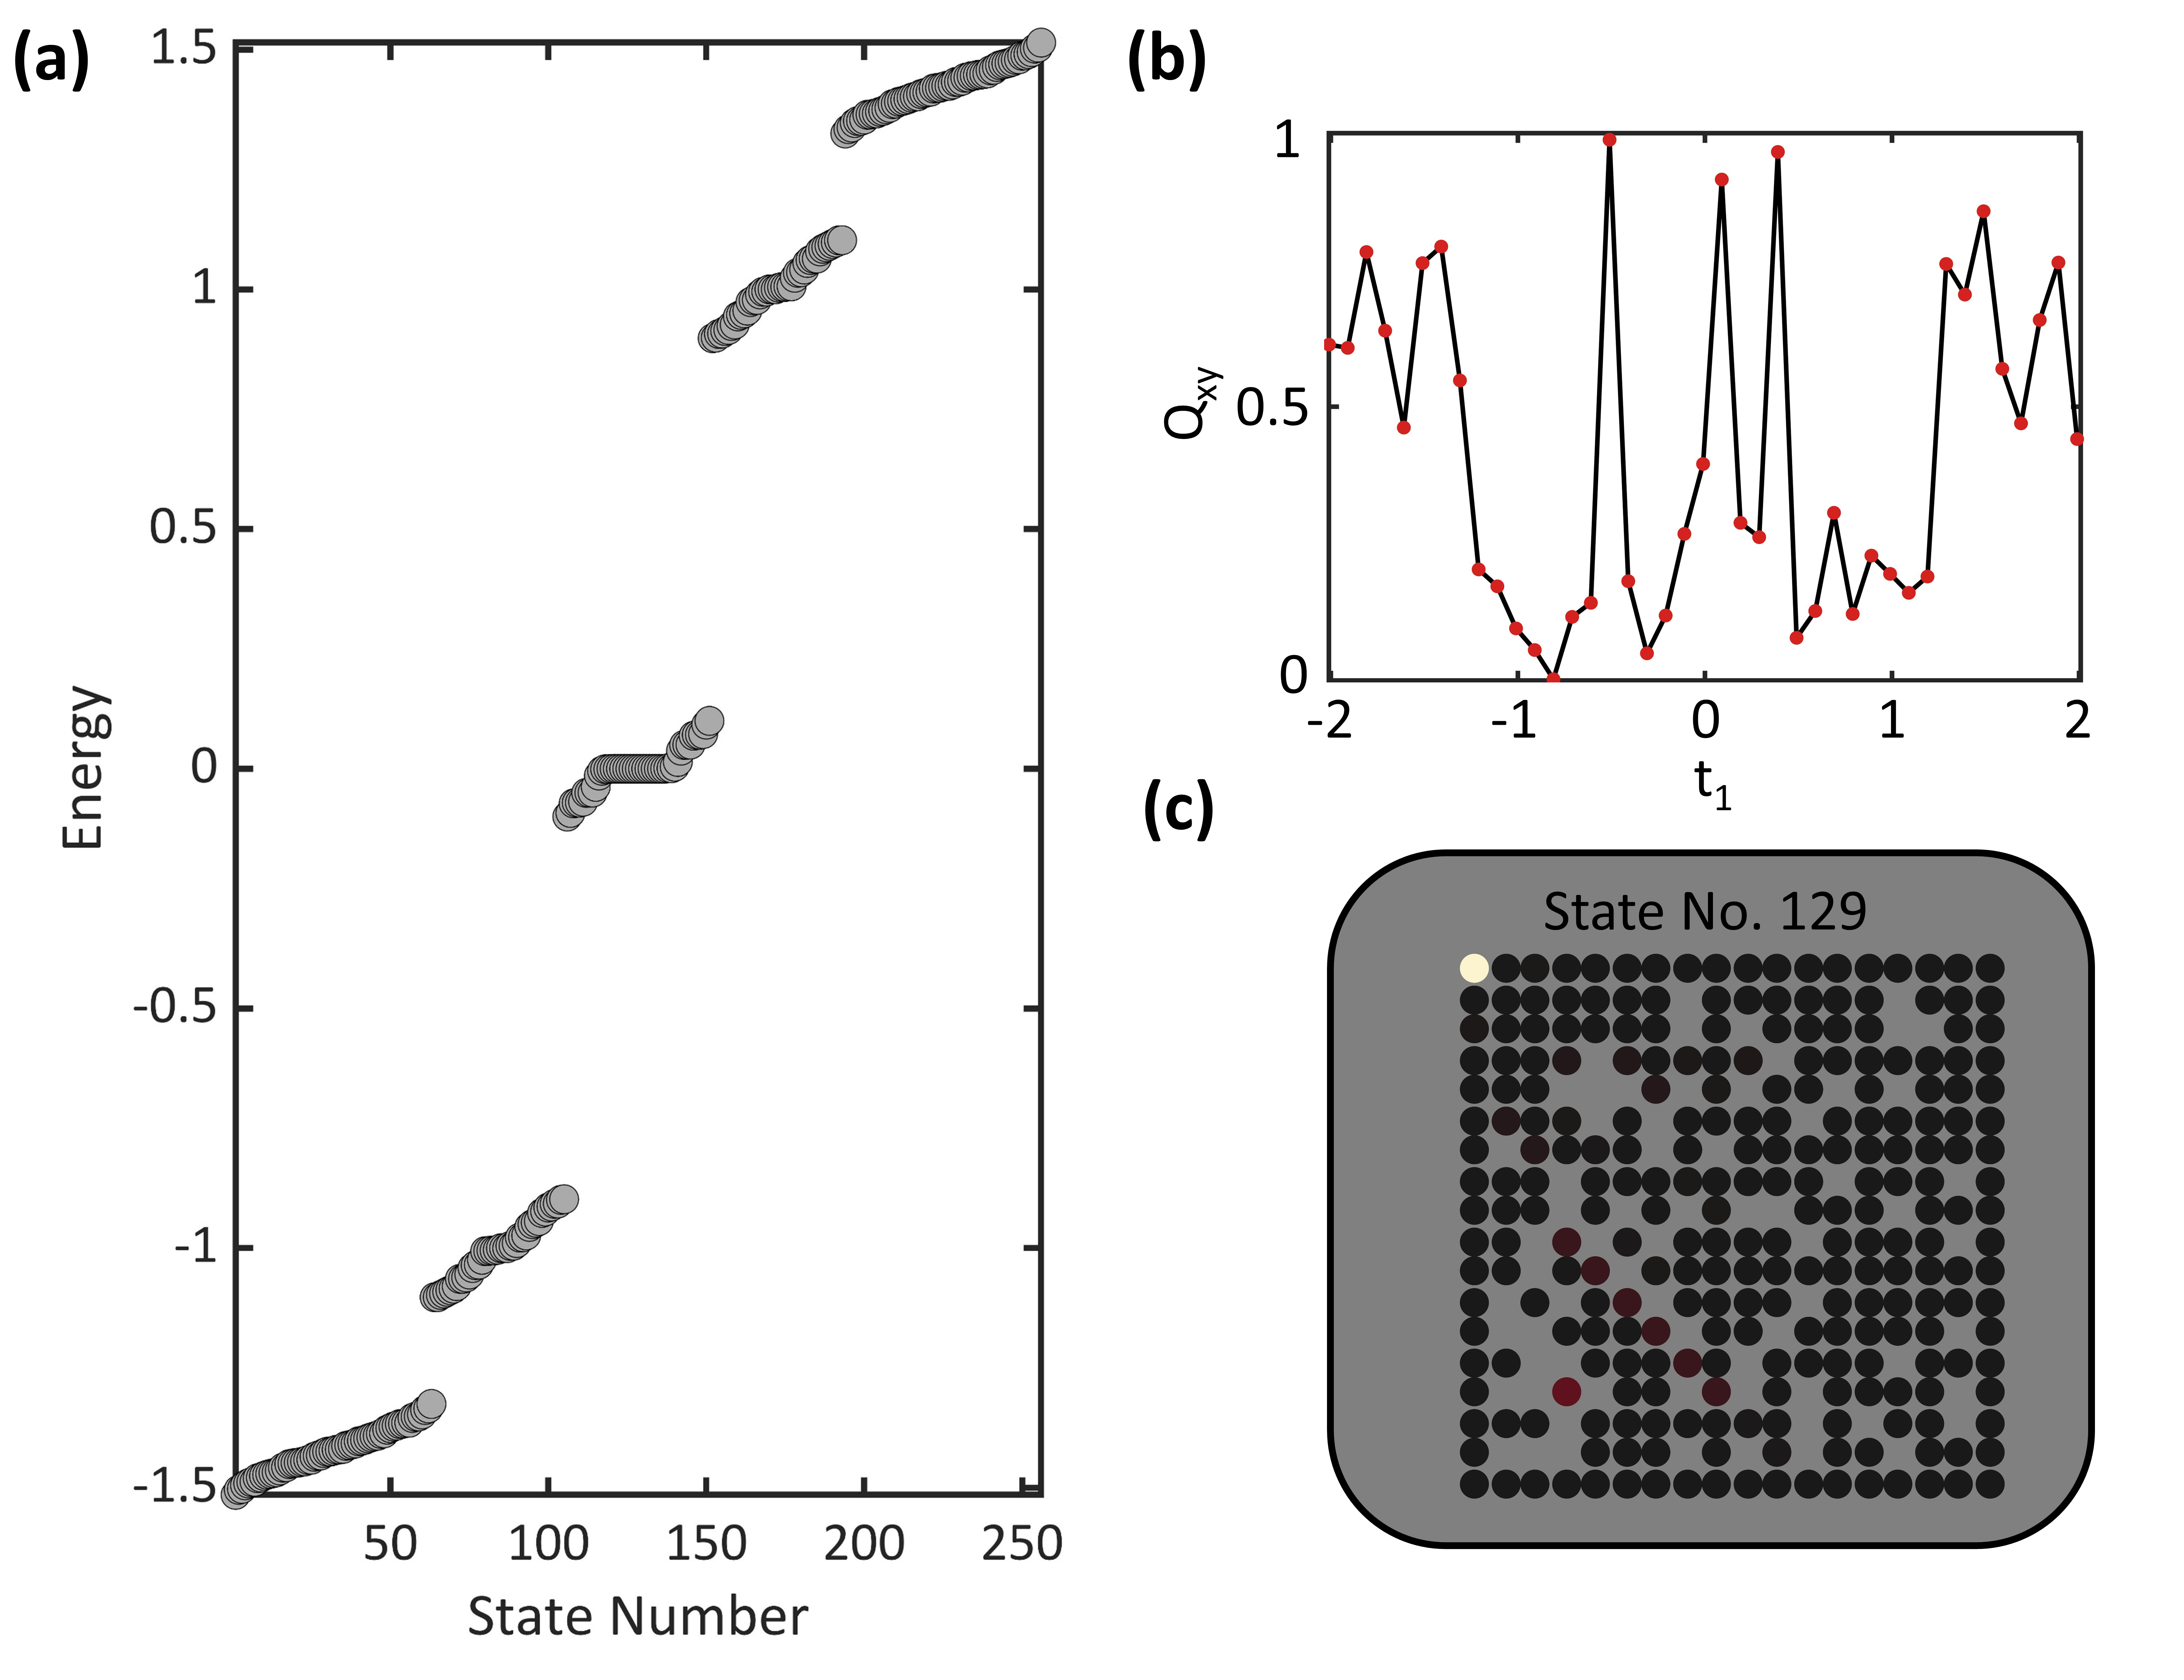
\includegraphics[width=0.5\linewidth]{figure/HOTITheo/RandDel.png}
    \caption{在方形晶格中随机删除站点}(a) 当 \( t_1=0.1 \) 时的能谱,其中方形晶格随机移除了 68 个站点。(b) 实空间拓扑不变量 \( Q_{xy} \) 随站点内跃迁 \( t_1 \) 变化的关系。(c) 在特定随机晶格实现中,编号 129 态的场分布。
    \label{fig:RandDel}
\end{figure}

需要注意的是,在图\ref{fig:RandDel}(c) 中绘制的左上角位置的 129 号态似乎是一个拓扑角态,但由于 \( Q_{xy} \) 未被量子化,它并非真正的拓扑态。因此,该系统在随机移除站点后,不再表现出自相似性,也不再具有丰富的拓扑角态。

总而言之,我们讨论了空间平移对称性破缺以及分形晶格代数对拓扑相变的影响,并发现空间平移对称性破缺是导致相区域收缩的主要原因。此外,我们表明分形模型中的高阶角态与随机移除站点的方形晶格具有显著不同的特性。

\subsection{分数电荷}
基于上述拓扑相变研究,我们在分形晶格的几何边界(外角)和自相似结构内部(内角)均观测到局域角态。这引发了一个关键问题:这些不同空间位置的角态是否具有相同的拓扑起源?为揭示其本质,我们引入分数量子化电荷理论\cite{li2020fractional,peterson2021trapped,liu2021bulk},通过谱电荷计算系统研究角态的拓扑属性。

\begin{figure}[htbp]
    \centering
    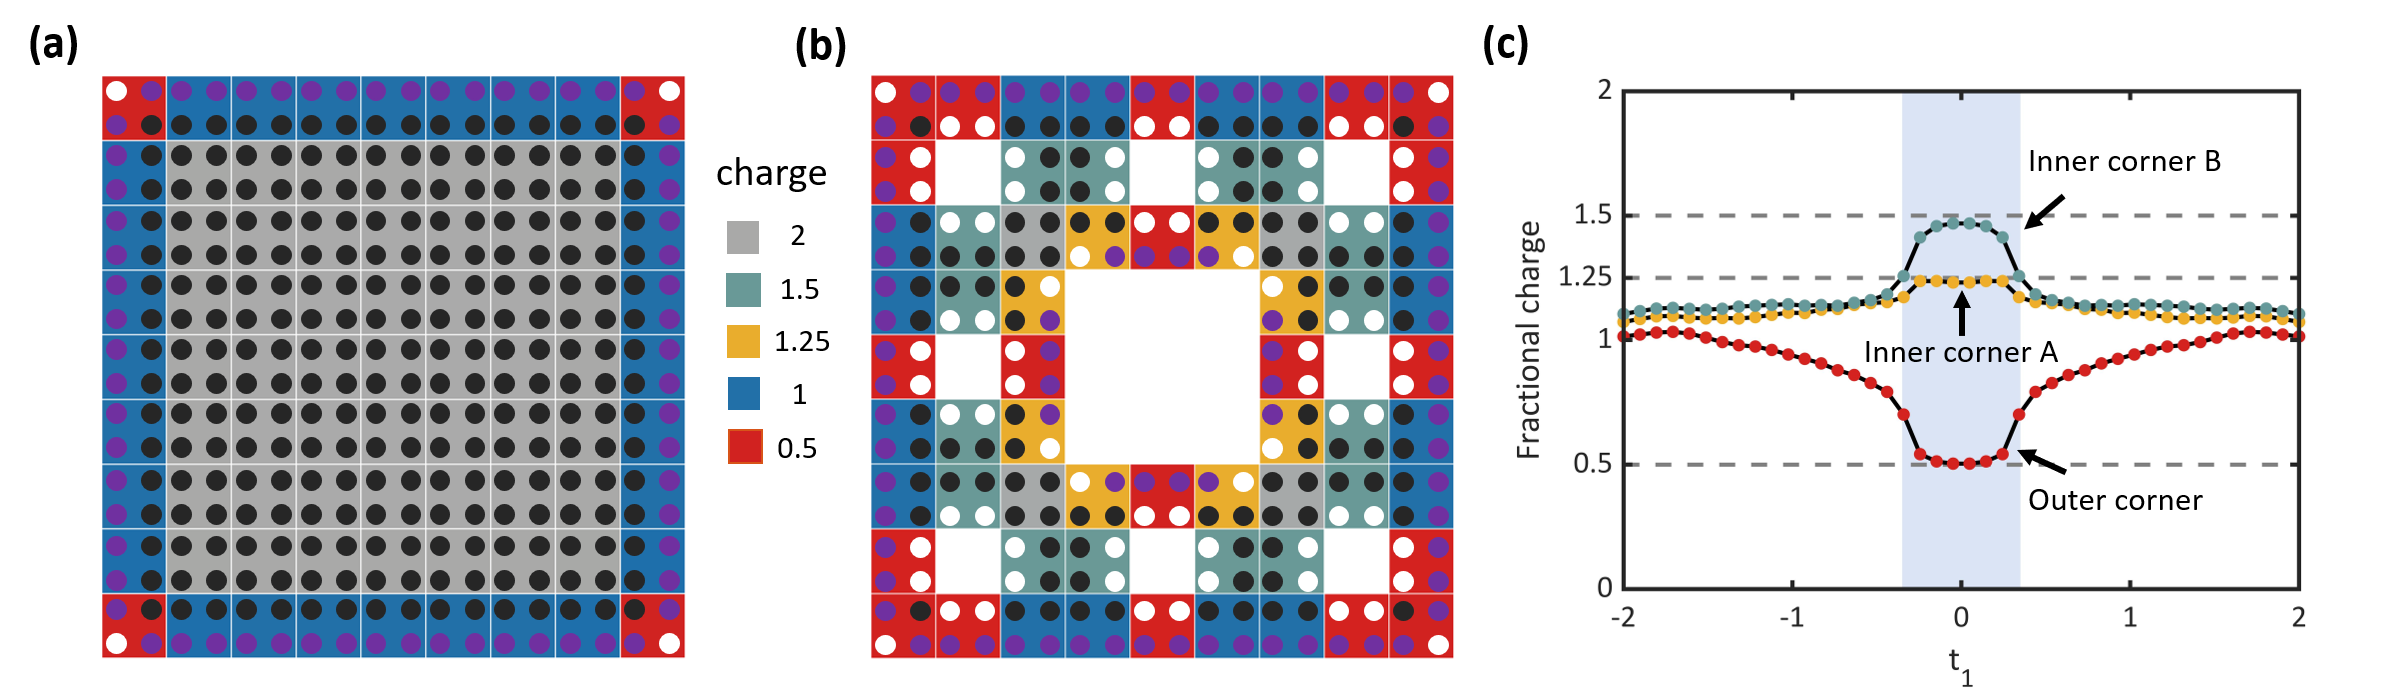
\includegraphics[width=1\linewidth]{figure/HOTITheo/Fractional.png}
    \caption{分数谱电荷}(a, b) 方形晶格与分形晶格的谱电荷。每个框覆盖一个单元格,其颜色表示电荷数。红色、蓝色、黄色、绿色和灰色框分别表示电荷数为 0.5、1、1.25、1.5 和 2。白色、紫色和黑色点分别对应晶格中的角态、边缘态和“体”态。(c) 外角态、内角态 A 和内角态 B 的电荷随站点内跃迁 \( t_1 \) 在 -2 至 2 范围内的变化关系,固定 \( t_2 = 1 \)。
    \label{fig:Fractional}
\end{figure}

在本节中,我们展示了方形晶格与分形晶格的谱电荷,如图\ref{fig:Fractional}(a, b) 所示。白色、紫色和黑色点分别表示晶格中的角态、边缘态和“体”态。我们计算了每个单元格内“体”态的局部态密度 (LDOS) 总和,该过程可以表示为:

\begin{equation}
q = \sum_{i \in \text{occupied}} \sum_{j \in \text{cell}} |\psi_i^j|^2
\end{equation}

其中,\( \psi_i^j \) 是每个单元格内第 \( j \) 个晶格点上第 \( i \) 个被占据的“体”态的波函数。我们通过不同颜色的框表示谱电荷,分别覆盖不同的单元格。红色、蓝色、黄色、绿色和灰色分别表示电荷数为 0.5、1、1.25、1.5 和 2。如图\ref{fig:Fractional}所示,二维晶格和分形晶格外角的分数电荷等于 0.5,这是高阶四极子绝缘体的重要特征。

在二维四极子 HOTI 中,电荷分别等于 0.5、1 和 2,对应于角态、边缘态和体态。然而,在分形晶格中,情况变得更加复杂。由于内角态分裂到两个最近的边缘站点,在内部角处出现了异常的空间电荷 \( q = 1.25, 1.5 \),如图\ref{fig:Fractional}(b) 所示。

值得注意的是,每个内角的两个角站点分别具有 0.25 的分数电荷,总计贡献 0.5 的分数电荷给每个内角。这一反直觉的结果的原因在于,跨越 \( 3\pi/2 \) 的内角可以将 0.5 的电荷分裂成两部分。

随后,我们计算了内角态和外角态的分数电荷随站点内跃迁的变化关系,以展示相变过程。固定站点间跃迁 \( t_2 = 1 \),并将站点内跃迁从 -2 变化到 2(如图 \ref{fig:Fractional}(c) 所示),所有三种角态仅在压缩的拓扑非平庸区域(蓝色区域)内被量子化。

由于内角和外角均存在非零的分数电荷,我们得出结论:所有角态均为拓扑非平庸态。尽管内角态和外角态的电荷不同,但它们的拓扑区域是相同的。

\section{高维分形晶格}
为了检验分形高阶拓扑绝缘体(HOTI)的普适性,我们在理论上构建了三维分形八极子拓扑绝缘体。

\begin{figure}[htbp]
    \centering
    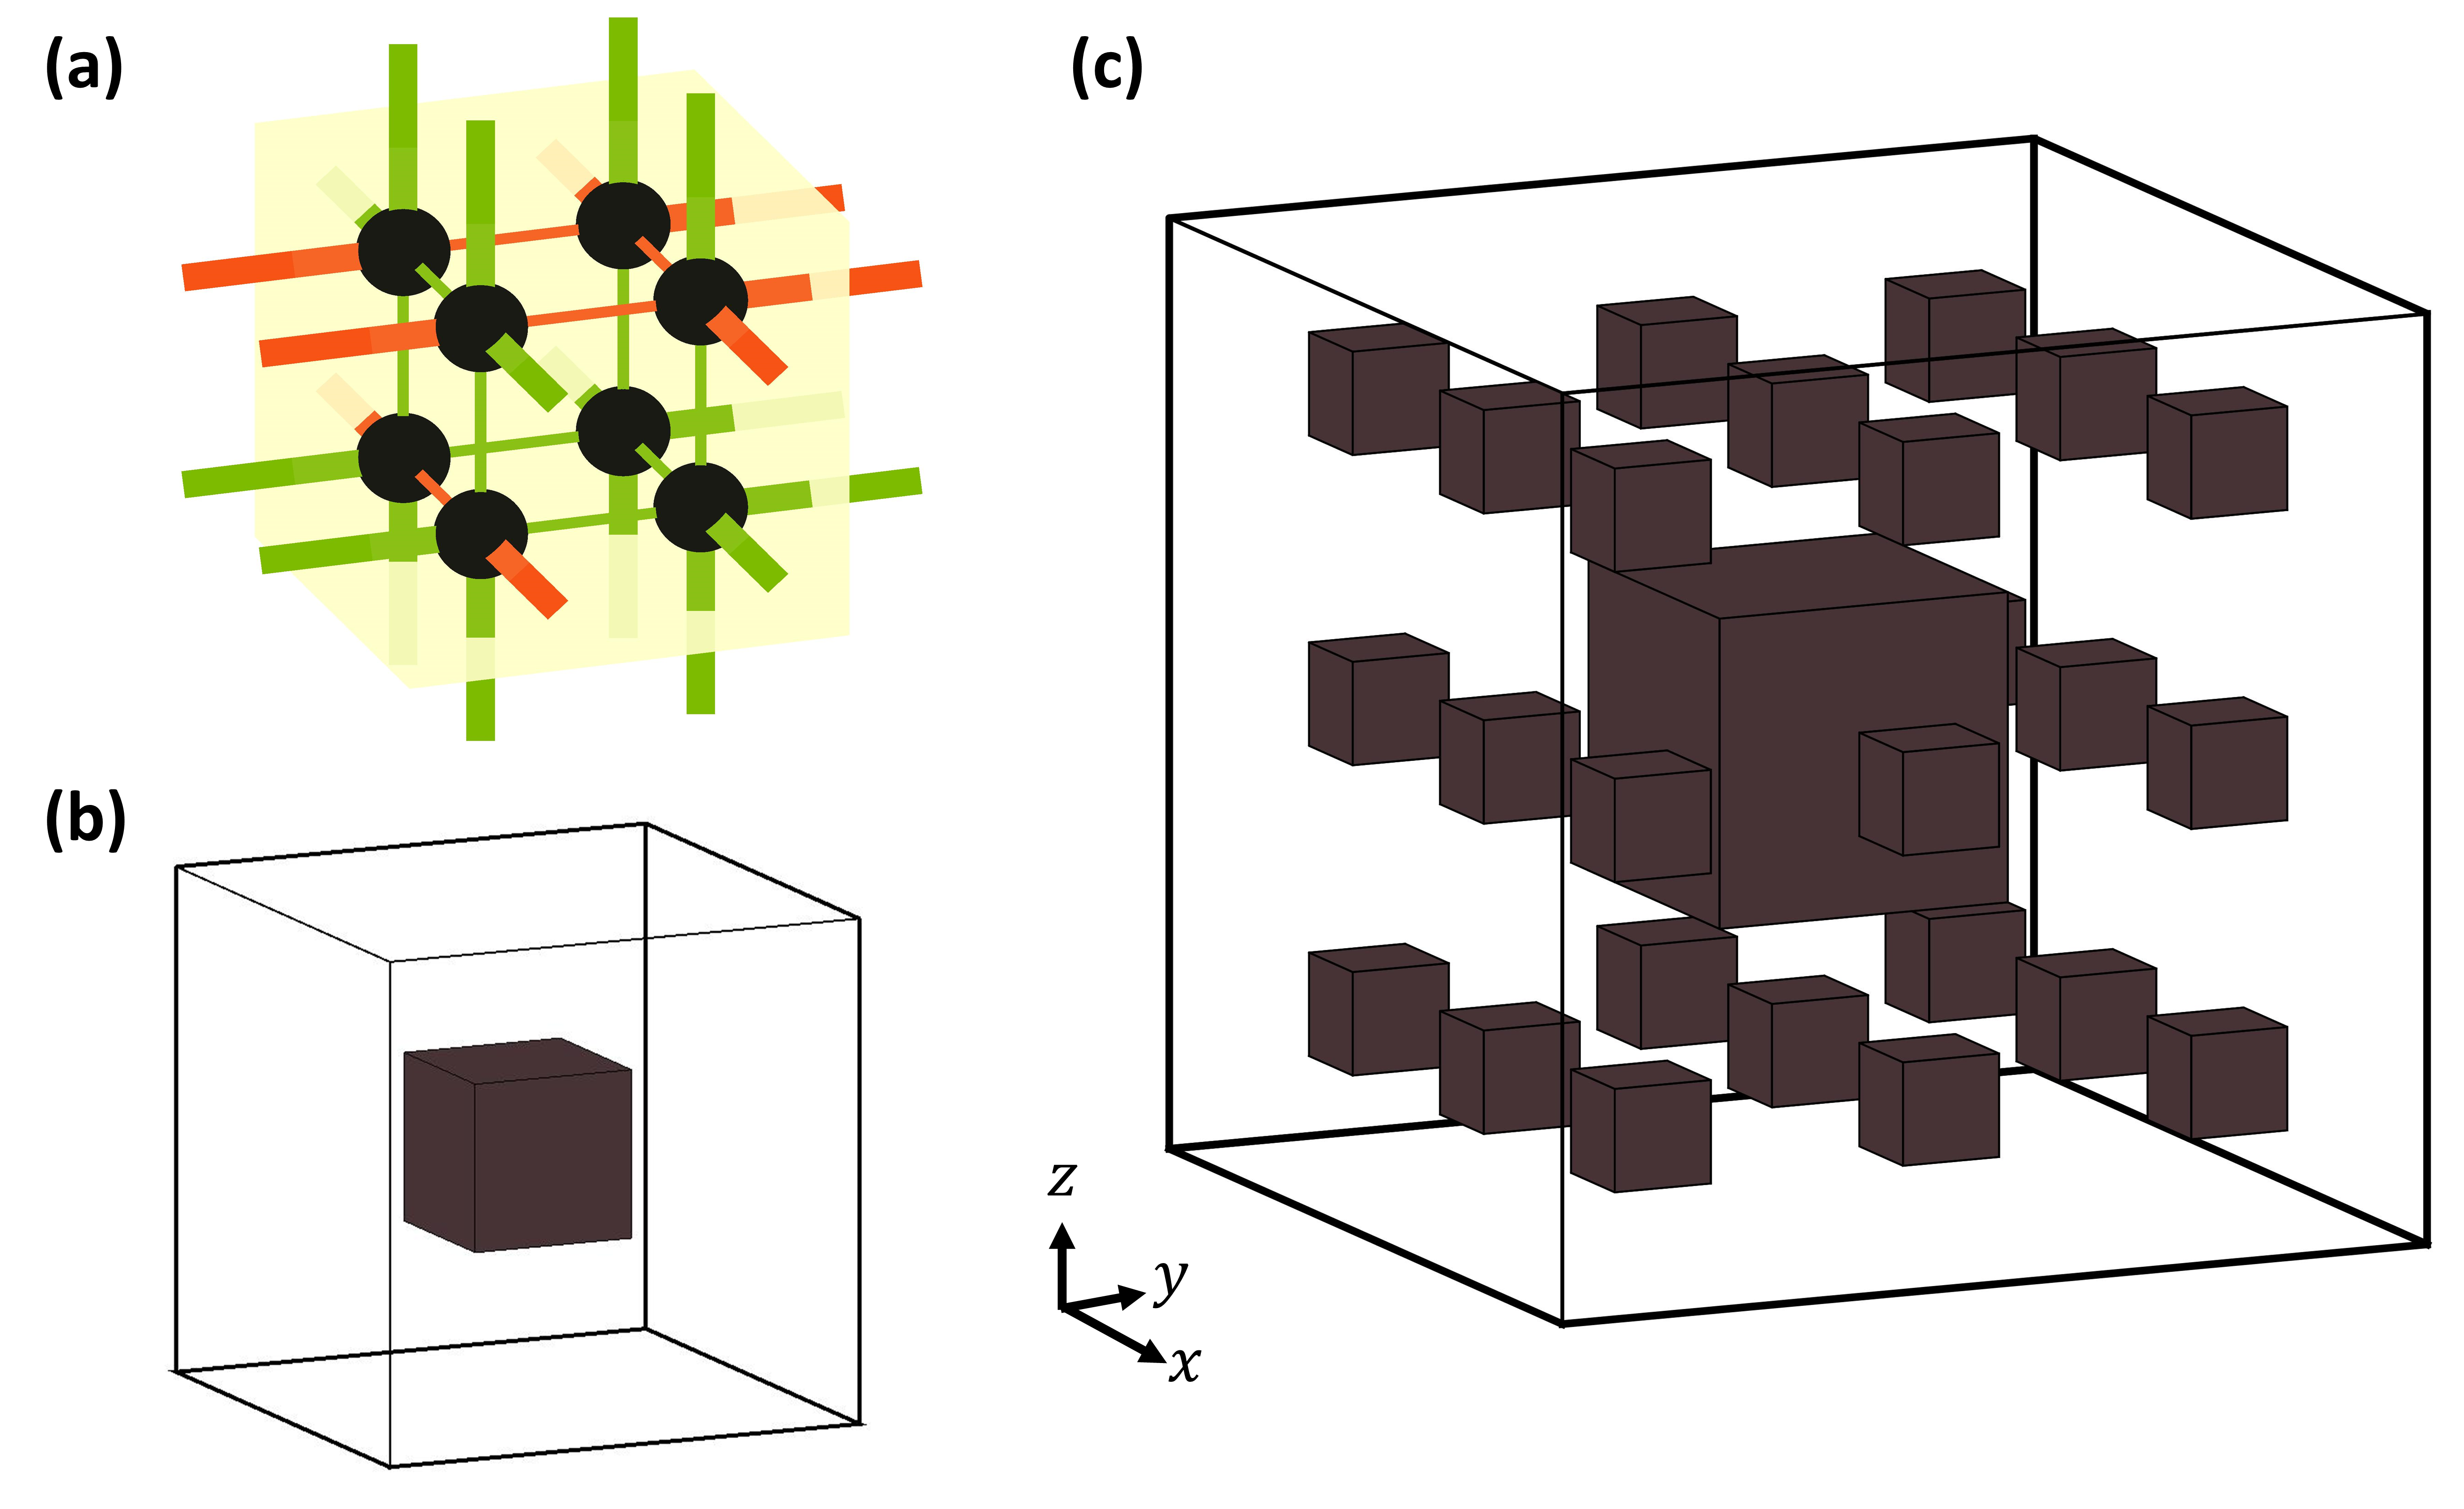
\includegraphics[width=0.5\linewidth]{figure/HOTITheo/3DLattice.png}
    \caption{高维分形晶格}(a) 分形晶格的最小元胞。(b, c) G(1) 和 G(2) 分形晶格。黑色立方体和白色部分分别表示真空和超原子。每一代 G(n) 的分形晶格由 G(n-1) 的 26 个副本组成。
    \label{fig:3DLattice}
\end{figure}

我们从传统八极子 HOTI 的元胞开始,如图\ref{fig:3DLattice}(a) 所示。红色(绿色)线表示正(负)跃迁,而粗(细)线分别表示站点间(站点内)跃迁。G(1) 晶格包含 26 个单元,如图\ref{fig:3DLattice}(b) 所示的白色部分。黑色立方体表示真空。G(2) 晶格如图\ref{fig:3DLattice}(c) 所示。由于每一代 Sierpinski 地毯的 G(n) 由 26 份 G(n-1) 组成,因此该分形系统的维度可以计算为:

\begin{equation}
D_s = \lim_{n \to \infty} \frac{\ln (N_s)}{\ln (N_l)} = \lim_{n \to \infty} \frac{\ln (26^n)}{\ln (3^n)} = \frac{\ln 26}{\ln 3} \approx 2.966
\end{equation}

能谱随站点内跃迁的变化关系如图\ref{fig:3DSpec}(a) 所示,插图为其放大视图。与前文的 1.893 维晶格类似,该 2.966 维晶格也存在外角态和内角态 A、B,分别用红色、橙色和黄色标记。灰色、蓝色和绿色曲线分别表示“体”态、表面态和边缘态。
\begin{figure}[htbp]
    \centering
    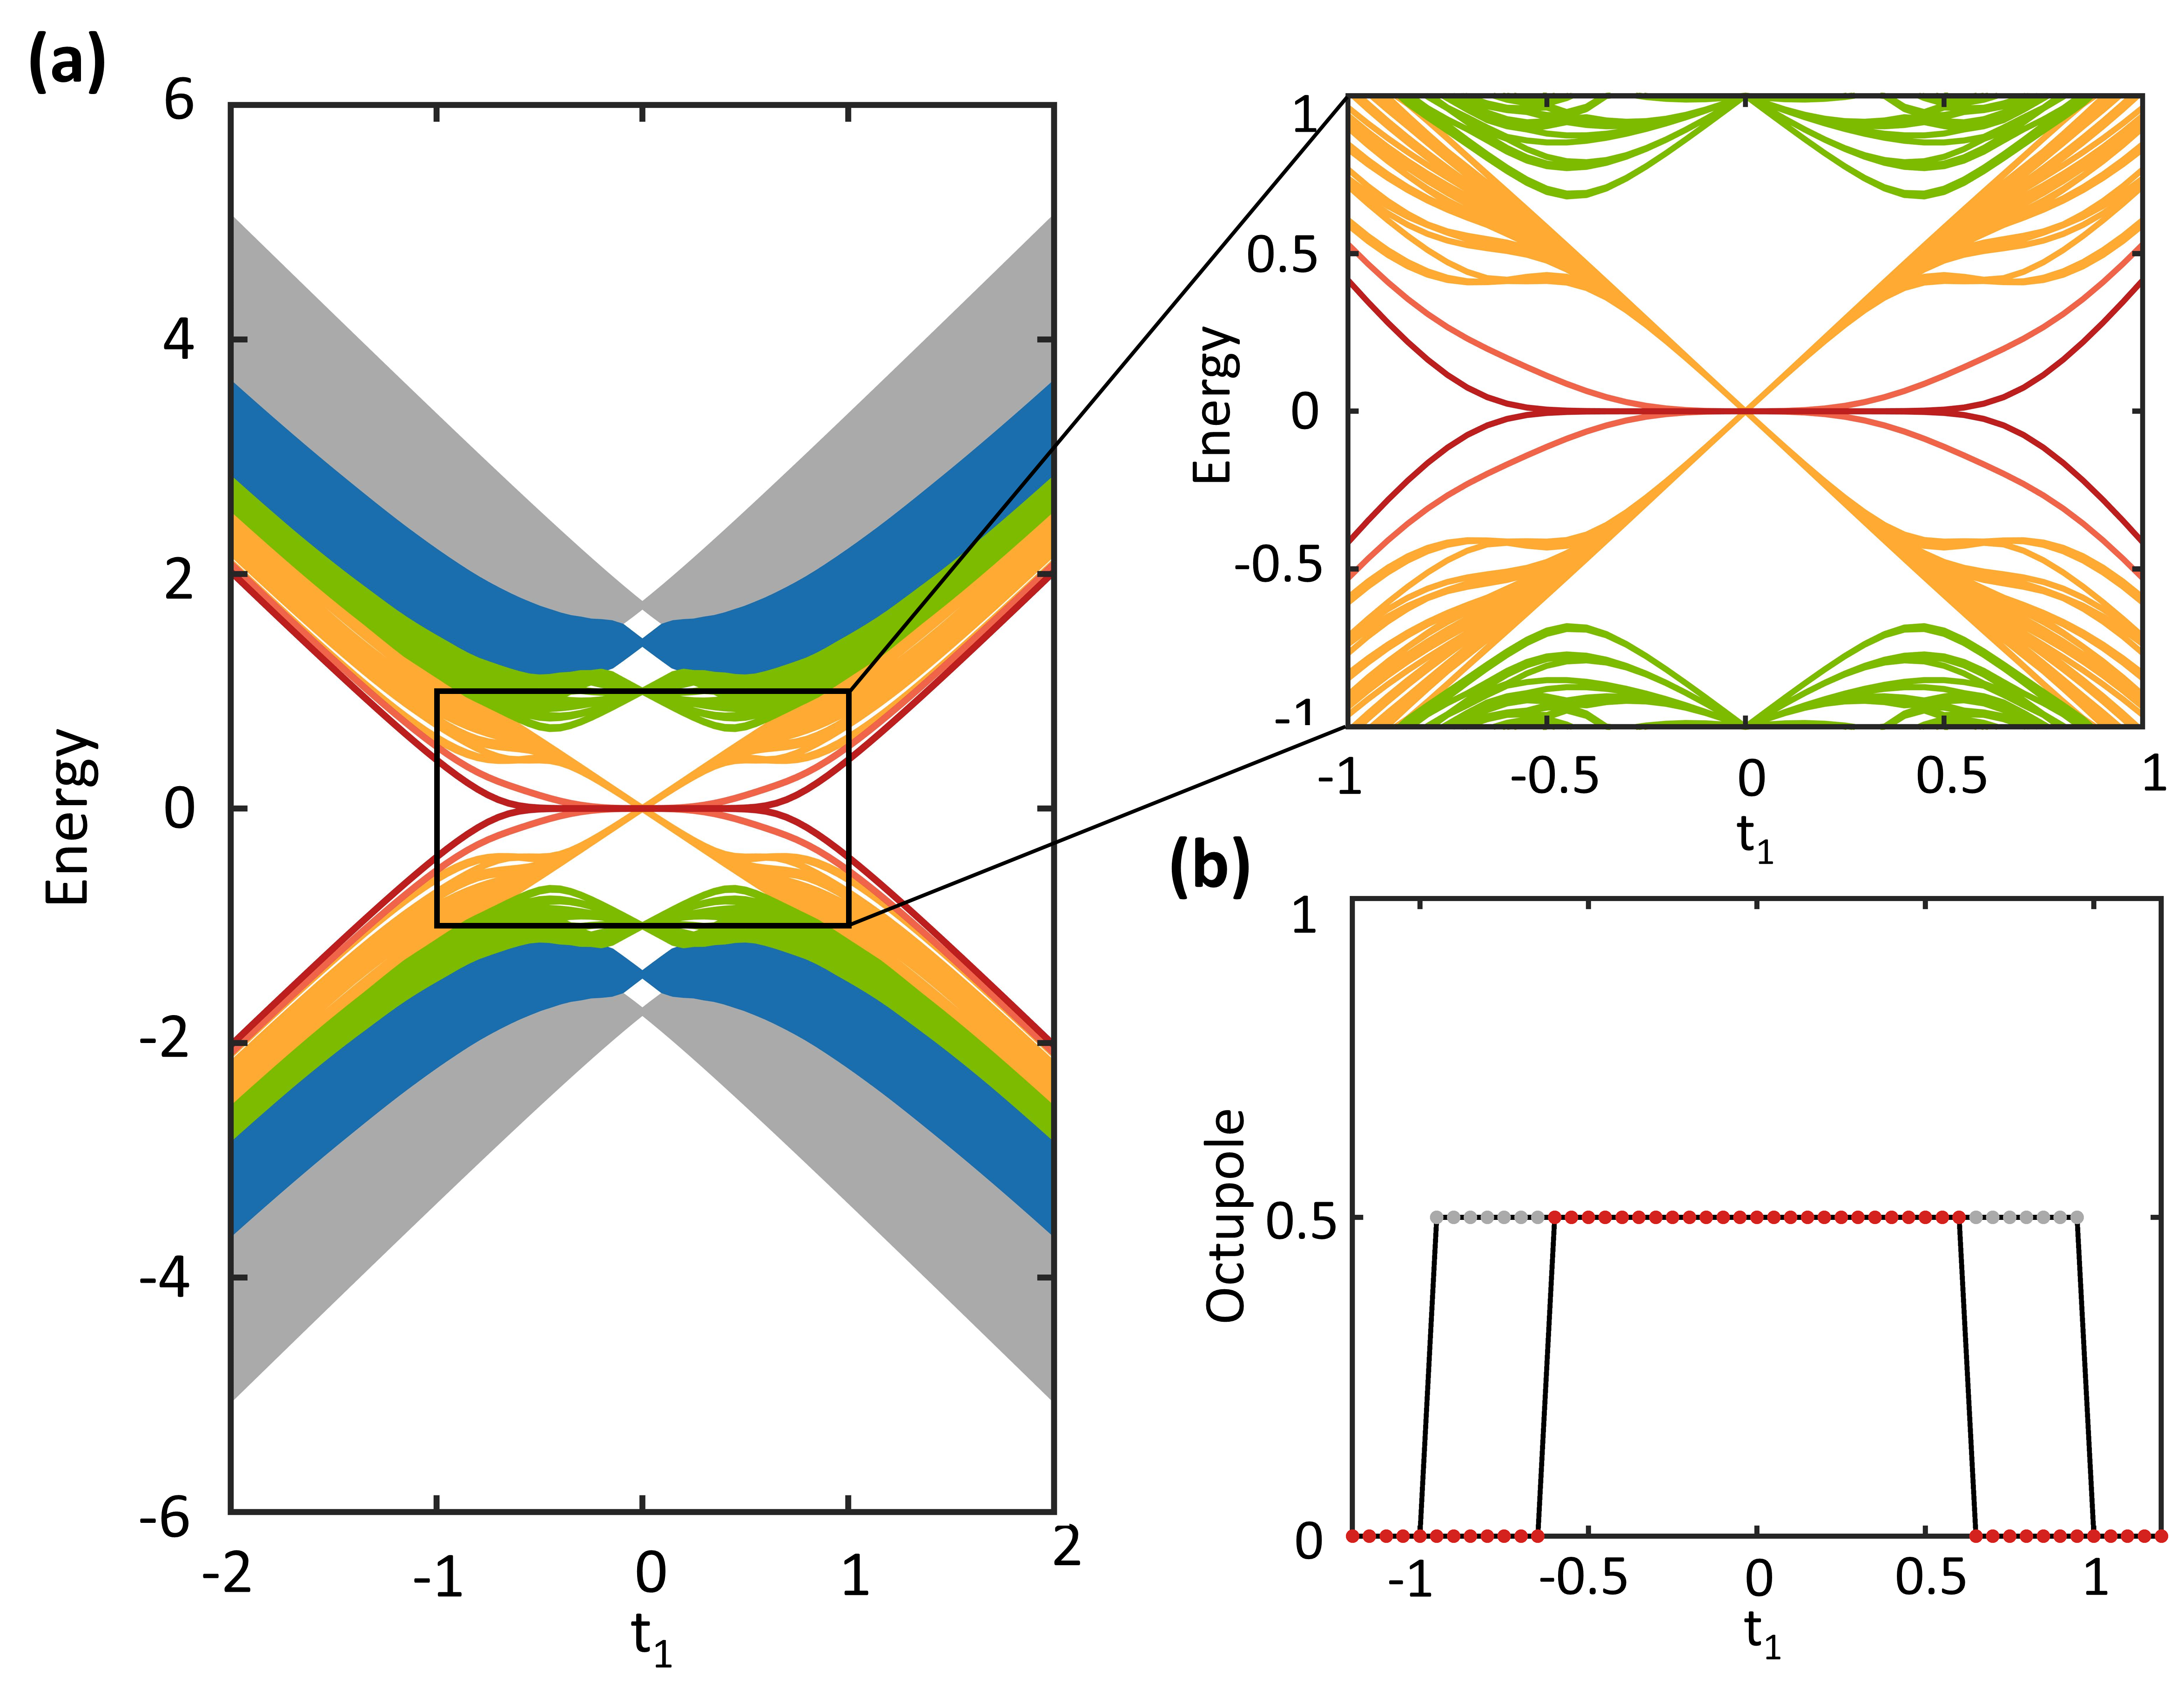
\includegraphics[width=0.5\linewidth]{figure/HOTITheo/3DSpec.png}
    \caption{分形“蝴蝶”结构与高维 SC 晶格的量子化八极矩}(a) 能谱随站点内跃迁 \( t_1 \) 的变化关系。红色、橙色和黄色线分别表示外角态、内角态 A 和内角态 B。铰链态、表面态和“体”态分别用绿色、蓝色和灰色标记。插图:(a) 的放大视图。(b) 计算得到的 2.966 维和 3D 晶格的八极矩分别由红色和灰色虚线表示。
    \label{fig:3DSpec}
\end{figure}
为了确定压缩的拓扑区域,我们计算了分形晶格中的八极矩:

\begin{equation}
O_{xyz} = \frac{1}{2\pi} \text{Im} \log \left[ \frac{\det \left( U^\dagger \hat{Q} U \right)}{\sqrt{\det \left(\hat{Q}^\dagger \right)}} \right]
\end{equation}

该计算方法类似于正文中的 \( q_{xy} \),唯一的区别是 \( Q \) 变为 \( \exp[i2\pi \hat{x} \hat{y} / (L_x L_y L_z)] \)。其中,\( L_x, L_y, L_z \) 分别表示晶格在 \( x, y, z \) 方向上的长度。

如图\ref{fig:3DSpec}(b) 所示,分形晶格和三维立方晶格中的拓扑不变量 \( O_{xyz} \) 随站点内跃迁的变化关系分别由红色和灰色点表示。在该分形晶格中,\( O_{xyz} \) 在 \( t_1 = 0.65 \) 处从 0 跳变至 0.5(小于立方晶格的对应值),并在 \( |t_1| < 0.65 \) 时保持 0.5,表明拓扑区域的压缩效应。

当 \( t_1=0.1 \) 时的能谱及其放大视图如图\ref{fig:3DState}(a, b) 所示,揭示了角态的自相似性。外角态、内角态 A 和 B 的总空间分布如图\ref{fig:3DState}(c) 所示。与 1.893 维晶格不同,2.966 维晶格的内角态分裂到三个最近的边缘站点,而非两个,这体现了高维晶格的特性。事实上,随着维度的增加,内角态会分裂成越来越多的部分,从而得到丰富的拓扑分数量子化电荷。此外,铰链态、表面态和“体”态的总空间分布如图\ref{fig:3DState}(d) 所示。
\begin{figure}[htbp]
    \centering
    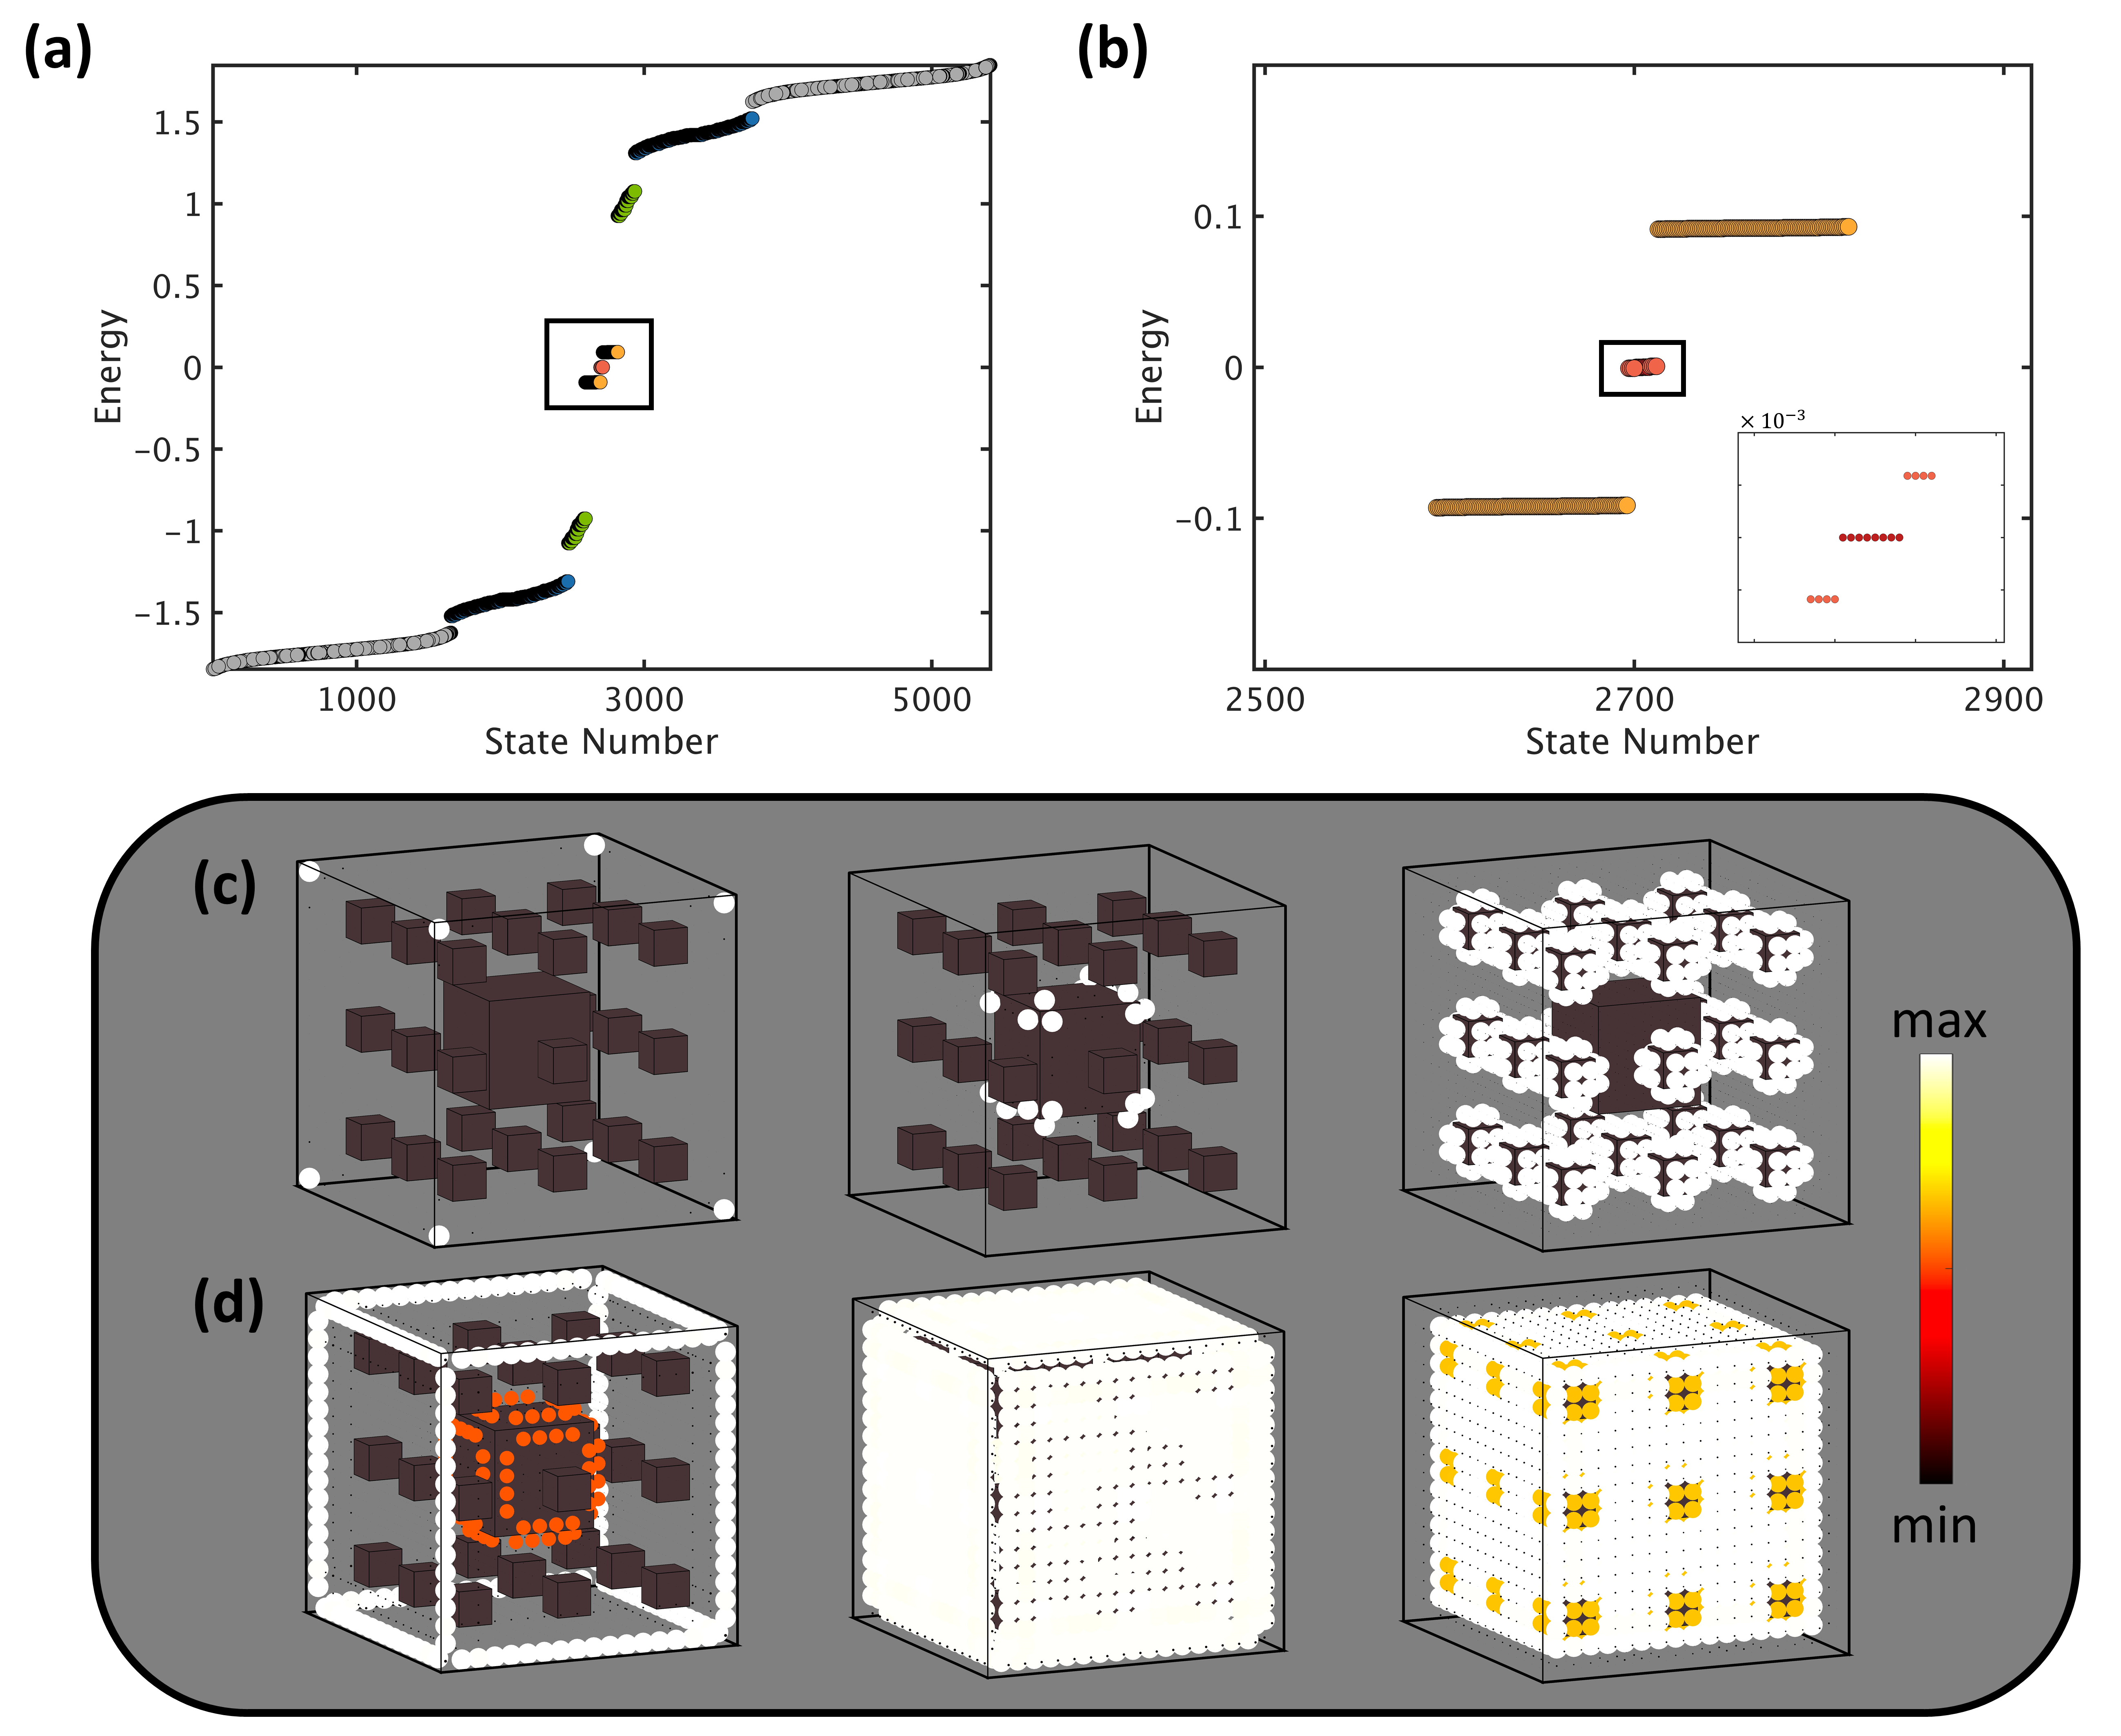
\includegraphics[width=0.75\linewidth]{figure/HOTITheo/3DState.png}
    \caption{有限分形晶格的能谱与本征态}(a, b) 当 \( t_1=0.1 \) 时的能谱及其放大视图。(c) 外角态、内角态 A 和 B 的总空间分布。(d) 铰链态、表面态和“体”态的总空间分布。
    \label{fig:3DState}
\end{figure}

\section{本章小结}
本章围绕分形 BBH 模型及其在分形晶格中的拓扑性质展开。首先,阐述了分形晶格的迭代生成,哈密顿量及其拓扑不变量,阐明了分形BBH模型的基本构建方案。接着,通过分析分形能谱和拓扑态,展示了分形晶格在能带演化过程中的分形“蝴蝶”能谱。

随后进入本章的核心内容:晶格与拓扑态的维度以及压缩的拓扑相图。通过计算拓扑内角态维度,发现内角态维度为1.89,其与晶格具有相同维度,其余维度为零。通过计算分形BBH模型的实空间拓扑不变量,笔者发现其拓扑相图被显著压缩为二维晶格的$35\%$。这种压缩性质不随晶格迭代变化。这种压缩性质也可以通过分数电荷验证。在分形晶格中,产生了电荷量为0.25和1.25的反常分数电荷,其标记了内角态的拓扑性质。通过计算其在不同参数下的结果,分数电荷标记了不同角态共享同样的压缩拓扑区域。为零的余维度以及压缩拓扑相图使得我们的分形晶格显著区别于传统的高阶拓扑绝缘体。

此外,本章还讨论了分形晶格在拓扑鲁棒性。分形晶格在手性无序和全随机无序下均显示了拓扑鲁棒性。但分形晶格对于无序的鲁棒性略低于二维晶格。最后笔者还展示了分形BBH模型的高维拓展,将之拓展到一个2.966维的分形晶格,其实现了一个八极子高阶拓扑绝缘体。